\documentclass[acmlarge]{acmart}

\usepackage{booktabs} % For formal tables


\usepackage[ruled]{algorithm2e} % For algorithms
\renewcommand{\algorithmcfname}{ALGORITHM}
\SetAlFnt{\small}
\SetAlCapFnt{\small}
\SetAlCapNameFnt{\small}
\SetAlCapHSkip{0pt}
\IncMargin{-\parindent}

% Metadata Information
\acmJournal{PACMHCI}
\acmVolume{9}
\acmNumber{4}
\acmArticle{39}
\acmYear{2010}
\acmMonth{3}
\acmArticleSeq{11}

%\acmBadgeR[http://ctuning.org/ae/ppopp2016.html]{ae-logo}
%\acmBadgeL[http://ctuning.org/ae/ppopp2016.html]{ae-logo}


% Copyright
%\setcopyright{acmcopyright}
%\setcopyright{acmlicensed}
%\setcopyright{rightsretained}
%\setcopyright{usgov}
\setcopyright{usgovmixed}
%\setcopyright{cagov}
%\setcopyright{cagovmixed}

% DOI
\acmDOI{0000001.0000001}

% Paper history
\received{February 2007}
\received{March 2009}
\received[accepted]{June 2009}


% Document starts
\begin{document}
% Title portion
\title{A Multifrequency MAC Specially Designed for Wireless Sensor
  Network Applications}
\titlenote{We can add a note to the title}

\author{Gang Zhou}
\authornote{This is the corresponding author}
\orcid{1234-5678-9012-3456}
\affiliation{%
  \institution{College of William and Mary}
  \streetaddress{104 Jamestown Rd}
  \city{Williamsburg}
  \state{VA}
  \postcode{23185}
  \country{USA}}
\email{gang_zhou@wm.edu}
\author{Valerie B\'eranger}
\affiliation{%
  \institution{Inria Paris-Rocquencourt}
  \city{Rocquencourt}
  \country{France}
}
\email{beranger@inria.fr}
\author{Aparna Patel}
\affiliation{%
 \institution{Rajiv Gandhi University}
 \streetaddress{Rono-Hills}
 \city{Doimukh}
 \state{Arunachal Pradesh}
 \country{India}}
\email{aprna_patel@rguhs.ac.in}
\author{Huifen Chan}
\affiliation{%
  \institution{Tsinghua University}
  \streetaddress{30 Shuangqing Rd}
  \city{Haidian Qu}
  \state{Beijing Shi}
  \country{China}
}
\email{chan0345@tsinghua.edu.cn}
\author{Ting Yan}
\affiliation{%
  \institution{Eaton Innovation Center}
  \city{Prague}
  \country{Czech Republic}}
\email{yanting02@gmail.com}
\author{Tian He}
\affiliation{%
  \institution{University of Virginia}
  \department{School of Engineering}
  \city{Charlottesville}
  \state{VA}
  \postcode{22903}
  \country{USA}
}
\affiliation{%
  \institution{University of Minnesota}
  \country{USA}}
\email{tinghe@uva.edu}
\author{Chengdu Huang}
\author{John A. Stankovic}
\author{Tarek F. Abdelzaher}
\affiliation{%
  \institution{University of Virginia}
  \department{School of Engineering}
  \city{Charlottesville}
  \state{VA}
  \postcode{22903}
  \country{USA}
}



\begin{abstract}
Multifrequency media access control has been well understood in
general wireless ad hoc networks, while in wireless sensor networks,
researchers still focus on single frequency solutions. In wireless
sensor networks, each device is typically equipped with a single
radio transceiver and applications adopt much smaller packet sizes
compared to those in general wireless ad hoc networks. Hence, the
multifrequency MAC protocols proposed for general wireless ad hoc
networks are not suitable for wireless sensor network applications,
which we further demonstrate through our simulation experiments. In
this article, we propose MMSN, which takes advantage of
multifrequency availability while, at the same time, takes into
consideration the restrictions of wireless sensor networks. Through
extensive experiments, MMSN exhibits the prominent ability to utilize
parallel transmissions among neighboring nodes. When multiple physical
frequencies are available, it also achieves increased energy
efficiency, demonstrating the ability to work against radio
interference and the tolerance to a wide range of measured time
synchronization errors.
\end{abstract}


%
% The code below should be generated by the tool at
% http://dl.acm.org/ccs.cfm
% Please copy and paste the code instead of the example below.
%
\begin{CCSXML}
<ccs2012>
 <concept>
  <concept_id>10010520.10010553.10010562</concept_id>
  <concept_desc>Computer systems organization~Embedded systems</concept_desc>
  <concept_significance>500</concept_significance>
 </concept>
 <concept>
  <concept_id>10010520.10010575.10010755</concept_id>
  <concept_desc>Computer systems organization~Redundancy</concept_desc>
  <concept_significance>300</concept_significance>
 </concept>
 <concept>
  <concept_id>10010520.10010553.10010554</concept_id>
  <concept_desc>Computer systems organization~Robotics</concept_desc>
  <concept_significance>100</concept_significance>
 </concept>
 <concept>
  <concept_id>10003033.10003083.10003095</concept_id>
  <concept_desc>Networks~Network reliability</concept_desc>
  <concept_significance>100</concept_significance>
 </concept>
</ccs2012>
\end{CCSXML}

\ccsdesc[500]{Computer systems organization~Embedded systems}
\ccsdesc[300]{Computer systems organization~Redundancy}
\ccsdesc{Computer systems organization~Robotics}
\ccsdesc[100]{Networks~Network reliability}

%
% End generated code
%


\keywords{Wireless sensor networks, media access control,
multi-channel, radio interference, time synchronization}

% DO NOT use this command unless you want to change
% the default behavior
% \authorsaddresses{Authors' addresses: G.~Zhou, Computer Science
%   Department, College of William and Mary, 104 Jameson Rd,
%   Williamsburg, PA 23185, US, \path{gzhou@wm.edu}; V.~B\'eranger,
%   Inria Paris-Rocquencourt, Rocquencourt, France; A.~Patel, Rajiv
%   Gandhi University, Rono-Hills, Doimukh, Arunachal Pradesh, India;
%   H.~Chan, Tsinghua University, 30 Shuangqing Rd, Haidian Qu, Beijing
%   Shi, China; T.~Yan, Eaton Innovation Center, Prague, Czech Republic;
%   T.~He, C.~Huang, J.~A.~Stankovic University of Virginia, School of
%   Engineering Charlottesville, VA 22903, USA; T. F. Abdelzaher,
%   (Current address) NASA Ames Research Center, Moffett Field,
%   California 94035.}

\maketitle

% The default list of authors is too long for headers.
\renewcommand{\shortauthors}{G. Zhou et al.}

\section{Introduction}
\label{sec:introduction}
Health-related IoT devices have been constantly attracting public attentions in recent years. According to a most recent report, the market of healthcare IoT reaches 41.22 billion USD in 2017 and is projected to grow to 158.07 billion USD by the year of 2022 \cite{healthiotmarket}. Besides the dramatic growing trend of the gross benefits, health-related IoT market is also prospering in the aspect of diversity of its products. Devices like smart wristbands and smart scales are two of the most well-known products in this area with which a user can monitor her health conditions varying from heartbeats, sleep level, to muscle mass or even bone mass.\\
\indent On one hand, users gain tangible benefits from the health-related IoT devices. On the other hand, however, users are also exposed to new and unknown risks. In January 2017, Department of Homeland Security (DHS) confirmed that nearly 465,000 implanted heart pumping devices, which are actively used in hospitals all-round the US, are vulnerable to remote attacks \cite{heartpump}. For example, hackers can remotely hack into a patient's defibrillator and trigger irregular heart rhythms which can cause a cardiac failure \cite{heartpump}. In September 2017, DHS issued a warning stating that approximately 4,000 wireless syringe infusion pumping devices are vulnerable to remote attacks \cite{infusionhack}. For instance, attackers can exploit a loophole to murder a patient by remotely giving the patient overdose infusion \cite{infusionhack}. As one can see from these cases, different from compromising traditional IoT devices such as smart hues or thermostats that results in system failures, compromising health-related IoT devices can not only cause leakage of a user's health information, but also directly jeopardize the user's life.\\
\indent Unlike the professional medical IoT devices mentioned above whose security problems have been gradually explored and addressed by more and more researchers, the security of home-use health-related IoT devices is seriously under-investigated. Therefore, a natural question is raised: are emerging home-use health-related IoT devices, which have a large amount of users, also suffer from similar security threats? To answer this question, we performed, to the best of our knowledge, the \emph{first} security analysis on home-use electroencephalography (EEG) IoT devices. The reason we chose EEG devices for our research is because they have a drastic growing market which is projected to reach 1.40 billion USD by the year of 2025 \cite{2025eegdevicemarket}. Moreover, EEG data is one of the most important and sensitive human health data that can reveal an individual's sensitive health conditions. Therefore, it is urgent and critical to investigate the security vulnerabilities of home-use EEG devices.\\
\indent In this paper, we studied the security of home-use EEG devices targetting the ThinkGear AM (TGAM) module manufactured by NeuroSky. NeuroSky is the most well-known manufacturer of the home-use EEG devices since it is the first company to make brain wave devices for home use in the world \cite{firsthomeeeg}, and it still holds the largest market share of home-use EEG devices \cite{neuroskymarket}. TGAM is the exclusive brain wave sensor ASIC module developed by NeuroSky; it was elected as TIME Magazine's 100 Best Toys of All Time and has a potential to be widely adopted by home-use EEG IoT manufacturers \cite{tgammarket}. In this research, we demonstrated that based on the security flaws of the EEG system framework due to the coarse-grained implementation, an attacker is able to construct two sets of easy-to-exploit PoC attacks, which contain 4 remote attacks and one proximate attack, to actively steal a user's brain wave data. A remote attack does not require the attacker to be close to the victim but a carefully crafted malicious program is needed. The proximate attack, on the other hand, does not require any malicious program, but it has to be launched within a certain distance away from the victim. %Thus, an attacker can freely choose any of these two sets of attacks based on real world situation. 
Because the security flaw exploited by our proximate attack exists in a mandatory step for the EEG data retrieval, all the 156 brain-computer interface (BCI) apps appearing in the NeuroSky App store, the official App store for TGAM devices, are vulnerable to this attack. We also conducted an empirical static binary analysis against all the 31 free apps in the NeuroSky App store and found that all of them are vulnerable to at least one remote attacks. %\\, with 32\% of them are vulnerable to both attacks. \\
\indent In addition, we studied the potential privacy leakage problem from the EEG data collected by the TGAM devices. It is well researched that rich-featured EEG signals collected by strict medical-use devices or research-use devices can reveal a user's sensitive information, e.g., focal disorders \cite{eegdiagnosis} \cite{dauwels2010diagnosis} and sleep levels \cite{nakamura2017automatic}. However, whether or not reduced-featured EEG data collected by home-use EEG devices can also pose similar privacy threats remains unexplored. In this paper, we proposed a novel recurrent convolutional neural network model (RCNN) targeting the reduced-featured EEG data collected by home-use EEG IoT devices to infer a user's focusing activities; our evaluation results over the realworld EEG data revealed that the proposed RCNN has an accuracy as high as 70.55\%, which significantly outperforms the other 11 most widely-used learning models.\\
%\indent Note that Martinovic \emph{et al.} \cite{martinovic2012feasibility} studied the possible side-channel leak from brain-computer interface (BCI) apps. Their work has the following two key differences from ours. First, we studied the security of home-use EEG IoT devices on both device-level and app-level, while they mainly studied the one on app-level. Second, the types of information inferred by their model are different the ones inferred by ours. Their model inferred a user's static information, e.g., the bank of a user's credit card, while our model inferred a user's active private information, e.g., the activity a user is currently focusing on. Third, Martinovic's \emph{et al.} leveraged EPOC device which is a research-use device and is not publicly available on the market for normal consumers as we will mention in section~\ref{sec:background}, even though the EPOC device collects much more features than home-use EEG IoT devices. While in our research, we took a step further to explore inference attacks on reduced-featured EEG data collected by home-use EEG IoT devices.\\
%\indent Note that Martinovic \emph{et al.} \cite{martinovic2012feasibility} studied the possible side-channel leak from brain-computer interface (BCI) apps. Their work has the following two key differences from ours. First, they focused on whether sensitive information can be deduced from the EEG data while we focused on how vulnerable the framework of home-use EEG IoT devices is. Second, Martinovic's \emph{et al.} leveraged the EPOC device which is a research-use device that is not publicly available in the market for normal home-use as we mention in section~\ref{sec:background}; the EPOC device collects much more features than home-use EEG IoT devices. While in our research, we took a step further to explore inference attacks on reduced-featured EEG data collected by home-use EEG IoT devices.\\
\indent \textbf{Our Contributions.} In summary, we have the following contributions in this paper:
\begin{itemize}
\item To the best of our knowledge, we proposed the first security analysis against home-use EEG IoT devices. We demystified the NeuroSky EEG system framework, which is not documented by the official NeuroSky documentations.

\item We identified the security flaws in the NeuroSky EEG system framework, based on which we constructed and fully implemented two sets of easy-to-exploit attacks to steal a user's brain wave data. %An attacker can freely choose any of these two sets of attacks according to real world situations. 
We also analyzed the BCI apps on the NeuroSky App store and discovered that all apps are vulnerable to the proximate attack, and that all the free apps are vulnerable to at least one remote attack. % one or both of the remote attacks: the malicious TGSP server attack and the malicious SDK attack.

\item We finally proposed a novel deep learning model to infer a user's activities based on the stolen reduced-featured EEG data with an inference accuracy as high as 70.55\%, which significantly outperforms other well-known learning models such as SVM, decision tree, and adaboost.
\end{itemize}

\indent \textbf{Paper Organization.} The rest of the paper is organized as follows. Section \ref{sec:related} outlines the most related work. Section~\ref{sec:background} introduces the preliminary knowledge on EEG, the types of different EEG devices, and our threat model. Section \ref{sec:framework} details the demystified EEG system framework. Section \ref{sec:attack} demonstrates the security flaws of the framework and the implementations of our attacks based on these flaws. Section \ref{sec:inference} presents our deep learning model for the reduced-featured EEG inference attack. Section \ref{sec:performance} reports the performance of our attacks and Section   \ref{sec:conclusion} concludes the paper.

%Finally, we wish that our research can serve as a security lesson to related parties and may offer an  to strengthen the security design for health-related IoT devices.

\section{Related Works}
\label{sec:related}
With the drastic development of home-use IoT systems, more and more studies were carried out to investigate the vulnerabilities of and attacks on smart home systems; on the other hand, research on sensitive personal information leak by the smart home IoT systems, especially the smart health systems, just started to thrive. In this section, we provide a brief overview on the most related research.\\
%
\indent \textbf{Health-related IoT Security.}
The security of health-related devices and systems have gained more and more attention in recent years due to the rapid development and the tight personal health connection. Eberz \emph{et al.} \cite{eberz2017broken} presented a systematic attack against the ECG biometrics and demonstrated its effectiveness by applying it to a successful commercialized ECG biometric product, the Nymi Band; they transformed the ECG signals collected on different ECG devices by a mapping function such that the signal collected on one device can be mimicked by the signal collected by a different device so that they can use arbitrary ECG signals for spoofing attacks. Different from their work, we focused more on the vulnerabilities of the home-use NeuroSky EEG system framework and the leak of the sensitive information revealed by the raw EEG signals; we developed 5 PoC attacks through which victim's activities can be surmised by analyzing the captured raw EEG signals.\\
\indent Rahman \emph{et al.} \cite{rahman2013fit} investigated the security and privacy issues of Fitbit; after reversely engineering the ANT protocol for data communications, they generated various attacks including the data capture attack, injection attack, denial of service attack, and so on; they also proposed possible defense mechanissms against the proposed attacks. Li \emph{et al.} \cite{li2011hijacking} demonstrated several security attacks on a popular glucose monitoring and insulin delivery system available on the market; by recovering the radio protocol, they proposed various attack scenarios and performed two types of attacks, passive attack and active attack; then they analyzed the attack scenarios and generated two defense schemes. Compared to the two pieces of research work mentioned above, besides the security of the health-related device itself, we also focused on the sensitive information leakage revealed by the captured EEG signals.\\
%
\indent Martinovic \emph{et al.} \cite{martinovic2012feasibility} explored a research-use EEG devices, EPOC, as a potential attack intermediary to infer private information about their users; with the EEG signals captured from EPOC, they calibrated the classifiers on a set of training observations; their results supported the hypothesis that personal sensitive information such as bank account and password might be unintentionally leaked. In contrast to their research, we chose a much more popular setting with a home-use EEG IoT device, which has much fewer electrodes than the ones of EPOC; instead of using the EEG device as an attack intermediary, we directly explored the security vulnerabilities of the EEG device itself; based on the weaknesses, we implemented 5 PoC attacks to steal the EEG data from the device; with the reduced-featured EEG signals, we can infer the user's activity at approximately 70.55\% accuracy.\\
\indent
Alongside the security study on health-related IoT devices, many work focused on building smart health systems and platforms. In \cite{solanas2014smart} \cite{yang2014health}, the authors discussed the concept of health-related smart city and the home-based wellness platform. Mirza \emph{et al.} \cite{baig2013smart} provided an overview on the design and modeling of the current smart health monitoring systems. Coincidentally, ISLAM \emph{et al.} \cite{islam2015internet} investigated the e-Health technologies and reviewed the existing advanced network architectures for e-Health; they also analyzed the distinct security and privacy features of the e-health structures, proposed an collaborative security model, discussed the innovations in health care contexts, and addressed various e-health policies and regulations.\\
%
\indent\textbf{More General IoT Security.}
General IoT security research has been thriving in recent years. Fernandes \emph{et al.} \cite{fernandes2016security} studied the Samsung's SmartThings smart home system by performing a combination of static analysis, runtime testing, and manual analysis on a dataset of 499 SmartApps and 132 device handlers downloaded in source form; they discovered 2 design flaws that lead to over-privileges even with the privilege separation module implemented, and found that the SmartThings event subsystem does not sufficiently protect the events that carry sensitive information; by exploiting these design flaws, they developed 5 PoC attacks targetting the SmartThings smart home system.  Costin \emph{et al.} \cite{costin2014large} managed to unpack and analyze 26,275 embedded system firmware images crawled from the Internet; with static analysis, they discovered a total of 38 previously unknown vulnerabilities in over 693 firmware images. M$\ddot{u}$ller \emph{et al.} \cite{muller2017sok} conducted a large scale analysis on the known printer attacks, and provided a general method for security analysis on printers; they also wrote a prototype software PRET to automatically evaluate 20 printer models and found that all of them are vulnerable to at least one of the known attacks. Manos \emph{et al.} \cite{antonakakis2017understanding} did a comprehensive analysis on Mirai's emergence and evolution. They analyzed how the botnet emerged, what classes of devices were affected, how Mirai variants evolved and competed for vulnerable hosts, and what types of attacks Mirai exploited.  Flavio \emph{et al.}  \cite{garcia2016lock} found that the entry systems of most VW Group vehicles maintain a few global master keys, which allows an adversary to clone a remote control and gain unauthorized access to a vehicle; they also presented a novel correlation-based attack on the Hitag2 rolling code scheme, which reveals the cryptographic key and thus enables an attacker to clone the remote control system. In contrast, our work focuses on the vulnerabilities of a specific type of home-use EEG system and its related sensitive information leakage. \\
%
\indent There also exsits research targetting the communication protocols of the IoT systems. For example, Ronan \emph{et al.} \cite{ronen2017iot} discovered a bug in the Touchlink part of the ZigBee Light Link protocol implemented by Philips, and compromised the global AES-CCM key used to encrypt and authenticate a new firmware so that an attacker can replace the benign firmware with a malicious one over-the-air; with all these findings they implemented a smart light bulb worm which automatically spreads and controls all the Philips smart lights. Our work is along with a similar line except that we further analyzed the captured EEG signals rather than just taking full control of the devices.


\section{Background}
\label{sec:background}

In this section, we first introduce the preliminary knowledge about electroencephalography (EEG). Then we briefly cover the differences among medical-use EEG devices, research-use EEG devices, and home-use EEG devices. Lastly, we demonstrate our threat model for the home-use EEG devices we are going to investigate. 

\subsection{Background Knowledge of Electroencephalography}
Human brain is consisted of thousands of nerve cells, also known as neurons. These neurons are constantly receiving, processing, and propagating information through electrical or chemical signals. The neurons are densely interconnected via a nervous structure with numerous synapses serving as intermediaries for passing or inhibiting electrical or chemical signals from one neuron to another neuron. There are two types of synapses: chemical synapse and electrical synapse. A chemical synapse converts an electrical activity from the pre-synaptic neuron into a chemical substance called neurotransmitter which is passed to the post-synaptic cell. Different from the chemical synaptic system, in the electrical synaptic system, the pre-synaptic neuron passes an electrical activity to the post-synaptic neuron through a special channel called gap junction where the electrical activity is converted into an ionic current and therefore inducing voltage changes between the pre-synaptic cell and the post-synaptic cell. Note that electrical synapses transmit signals much more rapidly than chemical synapses, and some synapses can act as both an electrical and a chemical synapse. Electroencephalography (EEG) is an electrophysiological method to detect and monitor the electrical activities of the generated voltages in the electrical synaptic system. Even though the electrical current generated by a single synaptic activity may be too tiny to be detected, fortunately, any human cerebral activity such as surprise, alertness, anger, and so on, usually requires more than 1,000 synaptic activities to complete, making EEG recording, which relies on physical measuring with electrodes attached to a scalp, possible. \\
\indent Even though EEG was introduced almost 80 years ago \cite{swartz1998advantages}, its potential is still actively researched nowadays. In clinical contexts, it has already been well known that EEG can help diagnose various focal disorders such as epilepsy, head injury, encephalitis, brain tumor, encephalopathy, memory problems, sleep disorders, stroke, and dementia \cite{eegdiagnosis}. In recent years, the ability of EEG to predict Alzheimer's disease is triggering more and more attention \cite{dauwels2010diagnosis}. In application contexts, besides the various games \cite{coyle2011eeg}, EEG has been actively studied for the fields such as sleep monitoring \cite{nakamura2017automatic} or even texting \cite{zhang2017converting}. On one hand, human beings can benefit from advancing technologies on EEG analysis; on the other hand, as one can readily see, if an individual's EEG data is not properly secured, it can cause severe threats to the individual's privacy.

\subsection{Medical-Use, Research-Use and Home-Use EEG}
According to our research, the current EEG methods and their corresponding devices can be classified into three categories based on the uses of EEG: for strict medical use, for research use, and for home use.

\subsubsection{Strict Medical-Use EEG}
The first type of EEG is intended for strict medical-use, which is mainly employed for focal diagnosis. The EEG data collected for this purpose usually has high dimensions of features. For example, traditional devices such as the large array magnetoencephalography system (MEG) employed by typical hostipals, has up to 125 electrodes attached to a patient's scalp for EEG data collection, which implies that each sample of the EEG data has at least 125 dimensions of features \cite{lantz2003epileptic}. Since these types of devices are intended for the extreme professional use only, they are usually not available in the markets for purchase.

\subsubsection{Research-Use EEG}
This type of EEG is intended mainly for research use, e.g., BCI research, which is often considered as a result of donwsampling the strict medical-use EEG. One of the most well-known research-use EEG systems is the BCI2000 \cite{schalk2004bci2000}. BCI2000 is a general purpose software system for brain-computer interface research whose device uses 64 electrodes covering a scalp to monitor EEG, which means that each collected data sample has at least 64 features. %The graph of the electrode positions of a BCI2000 device is shown in figure~\ref{fig:bci2000_pos}. 
Even though BCI2000 devices are not intended for strict medical use, they are still classified as professional devices which are costly and are not available for purchase publicly. A similar system is EPOC \cite{stytsenko2011evaluation} whose device has 14 electrodes attached to a scalp. This device again is not available for purchase in the markets. %The graph of the electrode positions of an EPOC device is shown in figure~\ref{fig:epoc_pos}.

\subsubsection{Home-Use EEG}
Home-use EEG is intended mainly for home-use applications, i.e., for lightweight medical-related uses. The device of this type of EEG only has three electrodes, with one attached to a person's left earlobe, one attached to the person's left forehead, and the last one attached to the person's right temple. %The graph of electrode positions of a home-use EEG device is shown in figure~ \ref{fig:homeuse_pos}. 
The market of this type of EEG is dominated by a company called NeuroSky \cite{NeuroSky}, which is the first company to commercialize home-use EEG devices and maintains the largest home-use EEG market share so far \cite{firsthomeeeg,neuroskymarket}. NeuroSky invented the PCB module, i.e., the ThinkGear AM (TGAM), which serves as a multi-mode sensor to collect EEG data, and the  EEG system framework for EEG data transmission. NeuroSky has an App store where users can purchase or download BCI apps. It also provides a software development kit (SDK) for developers to build BCI apps. All in all, NeuroSky establishes a mature platform for commercialization of the home-use EEG, and hence becomes the most popular brands in home-use EEG. Even though there exist other manufacturers for home-use EEG devices, most of their products leverage TGAM and adopt the EEG system framework. Compared with the previous two types of EEG devices, home-use EEG devices are much more affordable and are publicly available in many online markets such as Amazon. \\
\indent TGAM measures and offers 10 features of EEG, namely attention meter, mediation meter, delta, theta, low alpha, high alpha, low beta, high beta, low gamma, and high gamma. Besides attention meter and mediation meter which are calculated by previously studied algorithms, the other 8 types of data are traditional EEG waveforms and can be directly measured through different frequencies.
%
\begin{itemize}
  \item \textbf{Delta:} Delta is measured with frequency less than 4 Hz. It is often found during sleeping.
  
  \item \textbf{Theta:} Theta is measured with frequency ranging from 4 Hz to 7 Hz. It is often found during relaxation and meditation.
  
  \item \textbf{Alpha:} There are two types of alpha: low alpha which is measured with frequency ranging from 8 Hz to 9 Hz and high alpha which is measured with frequency ranging from 10 Hz to 12 Hz. Alpha is usually detected when eyes are closed or during relaxation.
  
  \item \textbf{Beta:} There are two types of beta: low beta which is measured with frequency ranging from 13 Hz to 17 Hz and high beta which is measured with frequency ranging from 18 Hz to 30 Hz. Beta is usually found during alertness or focuses. 
  
  \item \textbf{Gamma:} There are two types of gamma: low gamma which is measured with frequency ranging from 31 Hz to 40 Hz and high gamma which is measured with frequency ranging from 41 Hz to 50 Hz. Gamma is usually associated with multi-sensory processing, e.g., perception involving different senses such as sound and sight. 
\end{itemize}

Note that NeuroSky produces two types of EEG headsets: one is intended for personal computer (PC) only and the other can be used for both PC and mobile devices such as Android and iOS. However, we notice that the headset intended for PC only is much more popular than the one intended for both PC and mobiles since the purchase number of the former far exceeds the latter both on Amazon and Google Shop, and all the 156 apps on the NeuroSky official App store have a PC version but not all of them have a mobile version. On the other hand, the mechanism adopted by the mobiles is basically the same as the one adopted by PC. Therefore, in this paper, we conducted all our analysis against the PC platform.
  
\subsection{Threat Model}
In our adversarial model, attackers aim to steal brain waves of NeuroSky users and infer sensitive personal activity from these brain waves. For our remote attacks, we assume that an adversary is able to install a malicious program into a victim's PC and to execute the malicious program. There exist various ways for the adversary to accomplish this task. For example, the adversary can perform social engineering \cite{socialengineering}, or exploit the known remote code execution (RCE) vulnerabilities \cite{rce} and advanced persistent threat (APT) \cite{apt}. Note that these techniques are all viable and feasible, and have been widely adopted as attack vectors for compromising industrial systems \cite{socialengieerstat}\cite{aptstat}\cite{vulstat}. In this paper, we do not detail these procedures since they are out of the scope of our research. On the other hand, our proximate attack requires an adversary to be in a short-distance range, i.e., no more than 22 meters, away from the victim. However, the adversary does not need to have any access to any of the victim's devices. An adversary exploiting this attack can be a malicious neighbor, or a stalker who approaches the victim's home. If the victim wears the EEG headset device in a public area along with his laptop, the adversary can simply launch the attack in a nearby area, which could be some distance away and blocked by a few layers of walls, without triggering his suspicion. The adversary only needs to purchase related devices such as a GNU radio for a few hundred dollars.

%\begin{figure*}[h]
%        %\quad
%        \begin{subfigure}[t]{0.33\textwidth}
%          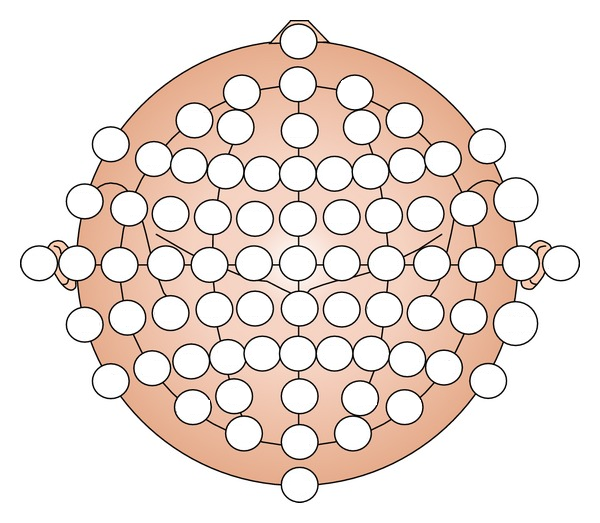
\includegraphics[width=0.975\linewidth]{bci2000_position.png}
%                \caption{BCI2000 device}
%                \label{fig:bci2000_pos}
%        \end{subfigure}
%        \begin{subfigure}[t]{0.33\textwidth}
%         \centering
%          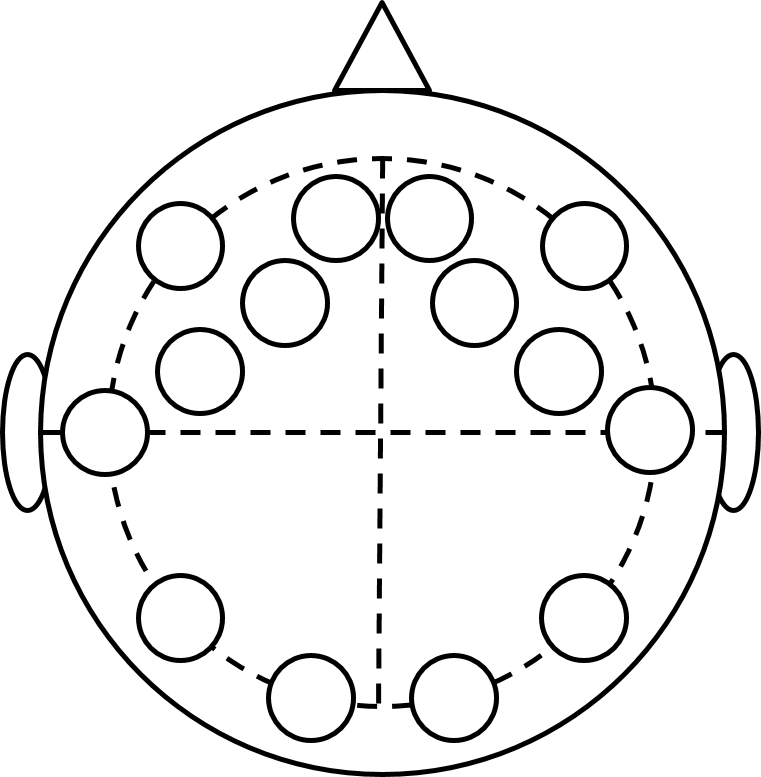
\includegraphics[width=0.8\linewidth]{epoc_position.png}
%                \caption{EPOC devices}
%                \label{fig:epoc_pos}
%        \end{subfigure}%
%        %\quad
%        \begin{subfigure}[t]{0.33\textwidth}
%          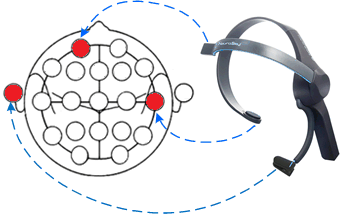
\includegraphics[width=0.975\linewidth, height=0.7\linewidth]{neurosky_position.jpg}
%                \caption{Home-Use EEG device}
%                \label{fig:homeuse_pos}
%        \end{subfigure}
%         \caption{Electrode positions in a human scalp of the EEG devices. A BCI2000 device has 64 electrodes, an EPOC device has 14 electrodes, while a home-use EEG device has only 3 electrodes.}
%         \label{fig:electrodepos}
%\end{figure*}

\section{Demystifying the EEG System Framework}
\label{sec:framework}

Before proceeding to introduce our new attack vectors, we first investigated the system framework adopted by the NeuroSky devices. As we mentioned in Section~\ref{sec:background}, most NeuroSky devices leverage TGAM, which employs the EEG system framework. Unfortunately NeuroSky does not explicitly publicize the specification details of the framework; therefore we conducted an empirical study by both reading the related documents such as the development guide and user guide published publicly, and conducting dynamic testing cases, to thoroughly recover the EEG system framework. We found that the EEG system framework can be separated into two sides, the user application side where high-level BCI apps reside and the headset side where brain waves are collected and transmitted. 

\subsection{User Application Side}
In the EEG system framework, the software-level implementations and operations are all integrated in the user's application side, whose hardware devices include the user's PC where BCI apps are running on and a radio frequency (RF) dongle serving as a communication bridge between BCI apps and the EEG headset, which is attached to the PC via a USB port. After exploring the developer's documentation, we recovered the sub-framework in the user application side and found that a BCI app running in the user's PC has the following two ways of retrieving the brain wave data: either from the standard software development kit (SDK) which retrieves the requested data from the RF dongle through the USB serial port, or via a pre-defined low-level socket protocol called ThinkGear socket protocol (TGSP). 

\subsubsection{EEG Data Retrieval through Standard SDK}
The EEG system framework provides a standard SDK for Windows operating systems so that Windows-based BCI apps can directly invoke API calls provided by the SDK for EEG data retrieval and all the necessary API functions are offered by a dynamic link library (DLL) binary file called \texttt{thinkgear.dll}. Unfortunately, the documentation lacks a systematic demonstration of the APIs in the DLL; therefore we reversely engineered the DLL and found that besides the DLL main entry function \texttt{DLLEntryPoint}, it exports 19 other API functions. After further exploration, we identified 4 functions that are mandatory to complete a EEG data retrieval; the other 15 functions are optional as they perform tasks such as writing a log stream, setting a baud rate, and reading a driver's version. The 4 mandatory functions are \texttt{TG\_GetNewConnectionId} through which the API caller is assigned an available integer as an identifier for a new connection to the RF dongle serial port, \texttt{TG\_Connect} which initializes a new connection that is bound with the provided connection id, \texttt{TG\_ReadPackets} which reads a raw packet through the RF dongle serial port, and \texttt{TG\_GetValue} which parses and returns a requested EEG data from a raw packet. The calls have to be made in the order of \texttt{TG\_GetNewConnectionId}, \texttt{TG\_Connect}, \texttt{TG\_ReadPackets}, and finally \texttt{TG\_GetValue}.

\subsubsection{EEG Data Retrieval through TGSP}
The EEG system framework also provides a low-level socket protocol, TGSP, for EEG data retrieval. TGSP can not only simplify the EEG data retrieval process since BCI apps do not need to go through the tedious SDK API calls, but also allow BCI apps to be implemented on different platforms other than Windows. TGSP adopts a server-client structure where there is an official server provided by NeuroSky, called ThinkGear Connector (TGC), which runs in the user's Windows platform, and BCI apps serve as clients sending requests to TGC and retrieving the desired data. \\
%
\indent The communications between TGC and the RF dongle is not complicated. As a matter of fact, the method leveraged by TGC to retrieve the EEG data from the RF dongle is fundamentally identical to the standard SDK; however, TGC integrates the API functions inside the TGC program with Windows .NET framework instead of making API calls to \texttt{thinkgear.dll}. The communications between TGC and BCI apps follows the following procedure: TGC first opens a fixed TCP port number \texttt{13854}, then a BCI app verifies itself with the TGC by sending a JSON request with the format shown below:
\begin{lstlisting}[language=json]
{"appName": "some app name", "appKey":"some app key"}
\end{lstlisting}
where the attribute \texttt{appName} is the name of the BCI app and \texttt{appKey} is a SHA-1 key of \texttt{appName} according to the documentation. Normally, the \texttt{appKey} should serve as a verification code for authentication. However, after a further exploration we noticed that the \texttt{appKey} serves merely as the app's identifier instead of a secret key assigned by the server; therefore, the whole verification process has little security implication. \\
%
\indent After the verification process, the BCI app can send a request with the following format to retrieve the EEG data from TGC:
\begin{lstlisting}[language=json]
{"enableRawOutput": true/false, "format": "Json/BinaryPacket"}
\end{lstlisting}
where \texttt{enableRawOutput} indicates whether or not TGC should return the raw voltage data from the three electrodes and \texttt{format} specifies whether TGC should return the data in the format of JSON or as a binary raw packet. \\
%
\indent If requested with the JSON format, TGC responds with the format shown below:
\begin{lstlisting}[language=json]
{"poorSignalLevel":n1,"eSense":{"attention":n2,"meditation":n3},"eegPower":{"delta":n4,"theta":n5,"lowAlpha":n6,"highAlpha":n7,"lowBeta":n8,"highBeta":n9,"lowGamma":n10,"highGamma":n11}}
\end{lstlisting}
where \texttt{poorSignalLevel} specifies the poorness level (ranging from 0 to 200, with 0 indicating a good signal while 200 indicating the off-head state) of the signal resulted from how properly the user wears the headset.\\
%
\indent If requested with the \texttt{BinaryPacket} format, TGC responds with raw packets following the structure shown in Table~\ref{tbl:basicpacket}. A packet begins with two \texttt{SYNCS} of value \texttt{0xAA} for each, followed by one byte indicating the length of the payload, the payload itself, and the 1-byte checksum for the payload. The payload is stacked with a number of \texttt{DataRow}s. A  \texttt{DataRow} is a special structure shown in Table~\ref{tbl:datarow} with a size of PLENGTH ranging from 1 to 256 bytes. It begins with an optional segment called \texttt{EXCODE} valued \texttt{0x55} with undefined size (undefined number of \texttt{0x55}s), followed by the 1-byte \texttt{CODE} indicating what type of data is passed, an optional 1-byte segment \texttt{VLENGTH} indicating the length of the value, and finally the value itself. The choices of \texttt{CODE} values are documented in \cite{tgsprawpacket}. Some of the most important ones include \texttt{0x02}, \texttt{0x04}, \texttt{0x05}, and \texttt{0x81}, representing poorness level of the signal, attention meter, meditation meter, and EEG power, respectively. 

%%%%%%%%% Basic Packet Structure
\begin{table}[]
\centering
\caption{TGSP Raw Packet Structure}
\label{tbl:basicpacket}
\resizebox{\columnwidth}{!}{
\begin{tabular}{llcccc}
\hline \hline
\multicolumn{2}{|r|}{SYNC}  & \multicolumn{1}{c|}{SYNC}     & \multicolumn{1}{c|}{PLENGTH}                                                      & \multicolumn{1}{c|}{PAYLOAD}                                                  & \multicolumn{1}{c|}{CHECKSUM}                                                                            \\ \hline \hline
\multicolumn{1}{|l|}{Content} & \multicolumn{1}{l|}{\texttt{0xAA}} & \multicolumn{1}{l|}{\texttt{0xAA}}  & \multicolumn{1}{c|}{\begin{tabular}[c]{@{}c@{}}Length of \\ payload\end{tabular}} & \multicolumn{1}{c|}{\begin{tabular}[c]{@{}c@{}}Series of\\ \texttt{DataRows}\end{tabular}} & \multicolumn{1}{c|}{\begin{tabular}[c]{@{}c@{}}Checks if the payload\\ has bit errors.\end{tabular}} \\ \hline
\multicolumn{1}{|l|}{Size}    & \multicolumn{1}{l|}{1 byte} & \multicolumn{1}{c|}{1 byte}                                                       & \multicolumn{1}{c|}{1 byte}                                                       & \multicolumn{1}{c|}{PLENGTH}                                                  & \multicolumn{1}{c|}{1 byte}                                                                              \\ \hline
                              &                             & \multicolumn{1}{l}{}                                                              & \multicolumn{1}{l}{}                                                          & \multicolumn{1}{l}{}                                                                                    
\end{tabular}
}
\end{table}

%%%%%% DataRow Structure
\begin{table}[]
\centering
\caption{Raw \texttt{DataRow} Structure}
\label{tbl:datarow}
\resizebox{\columnwidth}{!}{
\begin{tabular}{llccc}
\hline \hline
\multicolumn{2}{|r|}{(EXCODE)}                                  & \multicolumn{1}{c|}{CODE}                                                    & \multicolumn{1}{c|}{(VLENGTH)}                                                & \multicolumn{1}{c|}{VALUE}                                                       \\ \hline \hline
\multicolumn{1}{|l|}{Content} & \multicolumn{1}{l|}{\texttt{0x55}}       & \multicolumn{1}{c|}{\begin{tabular}[c]{@{}c@{}}Type of \\ data\end{tabular}} & \multicolumn{1}{c|}{\begin{tabular}[c]{@{}c@{}}Length of\\ Value\end{tabular}} & \multicolumn{1}{c|}{\begin{tabular}[c]{@{}c@{}}Value of\\ the data\end{tabular}} \\ \hline
\multicolumn{1}{|l|}{Size}    & \multicolumn{1}{l|}{Undefined} & \multicolumn{1}{c|}{1 byte}                                                  & \multicolumn{1}{c|}{1 byte}                                                   & \multicolumn{1}{c|}{VLENGTH}                                                  \\ \hline
                              &                                 & \multicolumn{1}{l}{}                                                         & \multicolumn{1}{l}{}                                                          & \multicolumn{1}{l}{}                                                            
\end{tabular}
}
\end{table}

\subsection{Headset Side}
In the EEG system framework, the TGAM chip in a headset collects user's EEG signals through the 3 electrodes and transmits the signals over-the-air through software defined radio (SDR). SDR is a novel radio technology in which the traditional components within the radio communication system, e.g., mixers, filter, modulator, and demodulator, which are used to be implemented in hardware, are realized by software. In our case, the TGAM in the headset encodes the EEG raw packets into radio signals, applies one types of modulation to the signals, and finally propagates the signals at a certain range of frequency; while the RF dongle takes care of receiving the signal from the predetermined frequency, filtering noises, demodulating signals, and finally decoding the EEG raw packets. Even though the SDR specification is not included in the user manual guide provided by NeuroSky, fortunately, we found that the Federal Communication Commission (FCC) ID of the NeuroSky home-use EEG IoT device, ``XG9MW1'', is printed on the device headset. According to per U.S. law, all products which emit radio waves have to register with FCC to maintain test reports of radio specifications. After exploring the headset's test report \cite{testreport} by searching the FCC ID, we found that the TGAM chip can operate on the frequency band ranging from $2419.9$ MHz to $2470.9$ MHz, and the modulation type is minimum shift keying (MSK) where messages are encoded into a sinusoid wave and a bit 0 and a bit 1 differ by half of a carrier period. %MSK has been widely adopted in industrial world for wireless communications; one of the most widely used MSK is called Gaussian minimum-shift keying (GMSK), which is a standard modulation method for GSM mobile phones.
\\
%
\indent However, as pointed out by the test report, a ThinkGear EEG device has an operable frequency range of $51$ MHz, which is too large for feasible analysis. In order to find the fine-grained center frequency via which the device is operating, we employed HackRF \cite{gadgetshackrf}, a SDR peripheral device capable of transimiting and receiving radio signals from $1$ MHz to $6$ GHz, and GQRX\cite{gqrx}, an open source SDR receiver powered by the GNU Radio. We conducted 30 experiments on 3 different NeuroSky EEG devices, 10 for each, and found that all devices in all experiments used the same center frequency with the same bandwidth: the approximate center frequency is $2458.4$ MHz with an occupied bandwidth of approximately $1$ MHz. A sample of the TGAM SDR wave is shown in figure~\ref{fig:sdrsample}.\\
%
\indent According to our experimental study and analysis described above, we concluded that the entire EEG system framework can be sketched as in figure~\ref{fig:tgframework}. It is consisted of four components: BCI apps, RF dongle, TGSP server, and TGAM. A BCI app is installed in the user's application side, and it has two ways of retrieving the user's EEG data when running, via either standard SDK or TGSP. If the BCI app requests an EEG data via the standard SDK, it directly communicates with the RF dongle through the USB serial port which returns the raw binary packet of the EEG data; if the BCI app requests an EEG data via the TGSP server (officially, the Thinkgear Connector), the server then retrieves the EEG data from the RF dongle likewise. Lastly, through SDR, the RF dongle receives the raw EEG data collected by the headset with the multi-modal sensor TGAM which employs three electrodes to measure the brain waves from a human scalp. The SDR has a center frequency roughly located at $2458.4$ MHz with an occupied bandwidth of approximately $1$ MHz.

\begin{figure}[!htb]
        \centering
        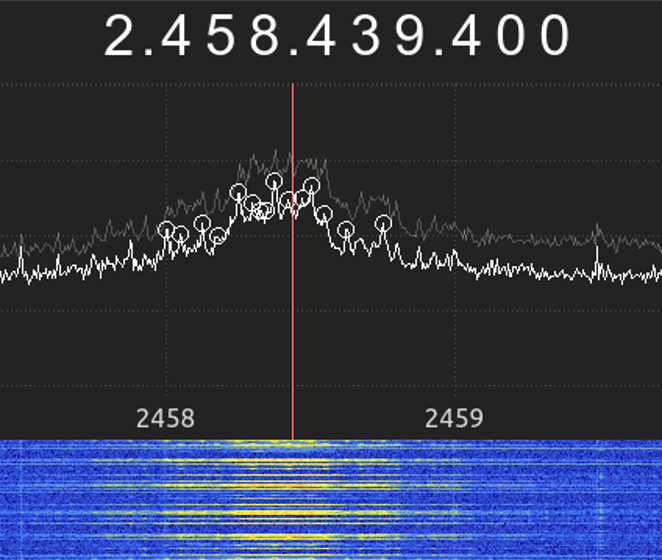
\includegraphics[width=\linewidth]{sdr_sample.png}
        \caption{A sample of the TGAM SDR wave. The center frequency is roughly $2458.4$ MHz and the occupied bandwidth is approximately $1$ MHz.}
        \label{fig:sdrsample}
\end{figure}

\begin{figure}[!htb]
        \centering
        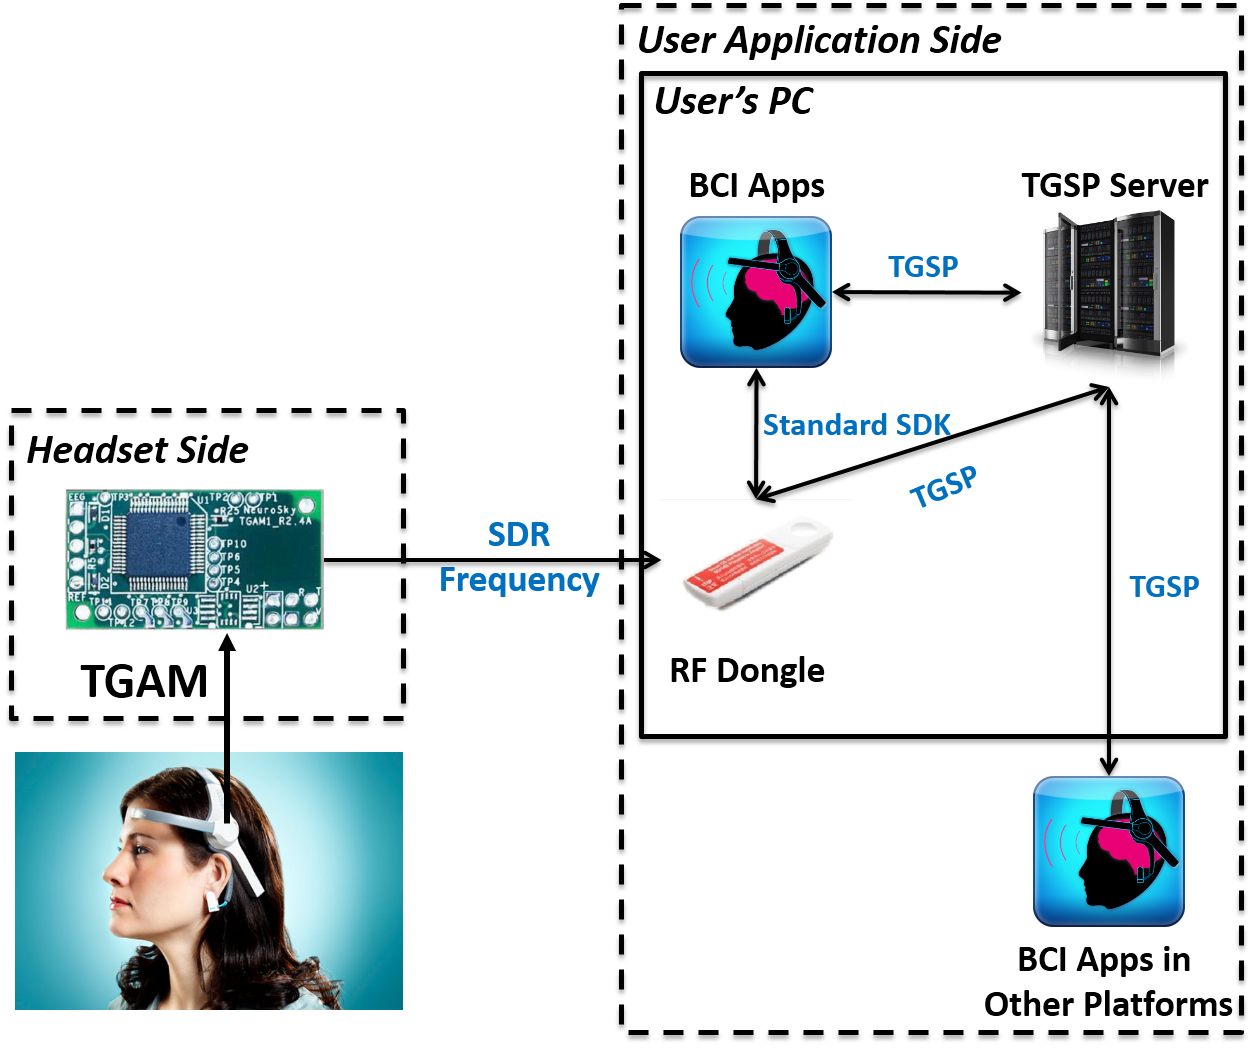
\includegraphics[width=\linewidth]{tgframework.png}
        \caption{The graph of the entire EEG system framework. A BCI app runs on a user's PC or other platforms within the user application side. If running on the user's PC, the BCI app can retrieve user's EEG data via either the standard SDK or TGSP. If running on a platform other than the user's PC, a BCI app can only retrieve the EEG data via TGSP. Both SDK and the TGSP server communicate with the RF dongle, which retrieves the EEG data from the user's headset through a SDR network.}
        \label{fig:tgframework}
\end{figure}

\section{Analysis and Implementation of Attack Vectors}
\label{sec:attack}

In this section, we detail our novel attack vectors targeting the EEG system framework we demystified in Section~\ref{sec:framework}. Our attack vectors can be classified as either remote attacks or proximate attacks. In a remote attack, an attacker can launch the attack without any constraint on how far he is away from the victim; however, a carefully crafted malicious program residing in the victim's PC side \emph{is} required to run. In a proximate attack, on the other hand, an attacker has to launch the attack within a certain distance away from the victim; however, \emph{no} malicious app is needed in this case. %Therefore, an attacker can freely choose any of the two types of attacks to launch based on different situations.

\subsection{Remote Attacks}
We came up with four remote attack cases based on the roles a malicious program plays in the EEG system framework: as a malicious BCI app, as a malicious TGSP server, or as a malicious SDK. We have fully implemented all these attacks. 

\subsubsection{Malicious Program as a BCI App}
The most straightforward attack is to install a malicious BCI app which secretly steals a victim's EEG data. As described in Section~\ref{sec:framework}, a BCI app can retrieve EEG data through either the standard SDK or TGSP. Correspondingly, there could be two approaches to implement such a malicious program. \\
\indent \textbf{Exploiting Standard SDK:} We first analyzed  if it is possible to implement a malicious BCI app which steals the victim's EEG data by exploiting the standard SDK. After an initial exploration, we found that if there is no other BCI apps running, our malicious app can successfully retrieve the EEG data; however, if there is another BCI app running, this method fails. We then  conducted dynamic debugging on the binary \texttt{thinkgear.dll} and found that when a BCI app calls \texttt{TG\_Connect}, \texttt{TG\_Connect} calls a sub function which invokes \texttt{CreateFileA} in Windows \texttt{kernel32.dll} and passes the fixed name of the RF dongle serial port, e.g., ``COM3'', as the file name to \texttt{CreateFileA}. Therefore, when a BCI app is accessing the serial port through SDK, another app would fail since \texttt{CreateFileA} would return the \texttt{ACCESS\_DENIED} error. Hence, through this method, a malicious app would have to terminate the benign program running a BCI app or the TGSP server (which is basically a BCI app), if any, in order to accomplish the attack. Intuitively, terminating a running benign app can trigger a victim's suspicion. Hence, a malicious app has to imitate the terminated benign app in every level, imposing a tremendous burden to the attacker. \\
\indent \textbf{Exploiting TGSP:} A relatively easy approach is to exploit TGSP; thus we examined the feasibility of a malicious BCI app accessing the EEG data through TGSP. As we mentioned in Section~\ref{sec:framework}, the TGSP server adopts a naive verification step merely for the purpose of distinguishing different apps. Therefore, we implemented a malicious app using C/C++ which generates a random string as the app name, constructs a SHA-1 digest for the app name, and sends these two pieces of information to TGC. If there is a conflict, our malicious app simply re-generates another random app name. It turns out that this attack functions normally.

\subsubsection{Malicious Program as a TGSP Server}
Instead of creating a malicious BCI app, we also created a malicious program which acts as a fake TGSP server and responds to benign BCI apps while retrieving the EEG data using the standard SDK. Note that even though this attack is refined based on the previous attack, it is more complicated since it needs to maintain TGSP so that benign BCI apps can run normally.\\
\indent In order for this attack to operate successfully, we first need to terminate the legitimate TGSP server, TGC, if it is running. TGC is not executed at the administrator level so that it can be terminated easily by calling the Windows Kernel API \texttt{TerminateProcess}. Then our malicious server maintains the TGSP specifications as we described in Section~\ref{sec:framework}. This attack is fully implemented in C/C++.

\subsubsection{Malicious Program as SDK}
Besides the attacks mentioned above, we also constructed an attack by modifying the standard SDK into a malicious one. In Section~\ref{sec:framework}, we identified the 4 mandatory API functions in \texttt{thinkgear.dll} to complete the EEG data retrieval. Among these 4 functions, the most important one is \texttt{TG\_GetValue} since it returns the requested EEG data. Hence, directly attacking this function in \texttt{thinkgear.dll} is the simplest and most effective way to steal the EEG data. \\
%
\indent In order to modify \texttt{TG\_GetValue}, we had to dig into the detailed specification of the function. \texttt{TG\_GetValue} is defined in the \texttt{thinkgear.h} header file; it has two parameters: an integer \texttt{connectionId} and an integer \texttt{dataType}, and returns a float value of the EEG data specified by \texttt{dataType}. We were interested in \texttt{dataType} and the returned float value while the \texttt{connectionId} has little implication to us. The \texttt{dataType} has 13 different values, namely the 8 EEG waveforms as we introduced in Section~\ref{sec:background}, the raw voltage value, the meditation meter, the attention meter, the signal poorness level, and the remaining battery power.\\
%
\indent Having identified our interested values in the function declaration, we next looked into the function body written in the \texttt{thinkgear.dll} to come up with a way to retrieve these values. As one can see in the binary codes of the function \texttt{TG\_GetValue} for a successful data return shown in figure~\ref{fig:getvaluebin}, the value of \texttt{dataType} is passed to \texttt{EAX} and the returned value is pushed onto the FPU floating point register stack \texttt{st0}; therefore, in order to steal these two values, we need to conduct a DLL injection attack.\\
%
\indent In Windows operating systems, there are basically two types of DLL injection attacks: dynamic DLL injection and static DLL injection. In a dynamic DLL injection attack, the malicious DLL is injected at runtime when the target process is running. %A malicious program leveraging this attack usually follows the following procedure: (1) first it creates a thread in the target process using \texttt{CreateRemoteThread}; (2) then it exploits \texttt{LoadLibrary} or the more advanced \texttt{ReflectiveLoader} to load the malicious DLL into memory; and (3) finally it writes to the target process using \texttt{WriteProcessMemory}. 
In a static DLL injection attack, an attacker can simply replace the benign DLL with a carefully-crafted DLL file. Under certain circumstances only dynamic injection can be applied, e.g., the target DLL has system-level privilege which prevents a third-party program from directly modifying it; and in other cases, static injection may be possible. Static injection is more effective since dynamic injection requires the target process to be running, and the malicious program has to know the process id of the target process. In our case, \texttt{thinkgear.dll} does not require the system-level privilege; thus we used static injection for our attack.\\
%
\indent Having decided to use static DLL injection, we then dug into the details of altering the benign \texttt{thinkgear.dll} into a malicious one. As discussed above, we need to steal two values, \texttt{EAX} and \texttt{st0}; therefore, we crafted a shellcode that can create a TCP client socket via which these two values are passed to our malicious server. In addition, after looking into the PE header of \texttt{thinkgear.dll}, we found that the virtual size and the raw size of the \texttt{.text} section are 70,692 (\texttt{0x11424}) bytes and 71,168 (\texttt{0x11600}) bytes, respectively, meaning that we need to squeeze the size of our shellcode to be less than 476 bytes since otherwise we have to either put the shellcode into other sections such as \texttt{.data}, which may fail to be executed due to data execution protection (DEP), or modify the PE header of \texttt{thinkgear.dll}. Fortunately, we were able to implement a shellcode with a size of 275 bytes, which can steal the two values and pass to our malicious server via a TCP connection. The address for injecting the shellcode begins at \texttt{0x11824} since the raw offset for \texttt{.text} is \texttt{0x400} (\texttt{0x11824}=\texttt{0x11424}+\texttt{0x400}). The injected shellcode is shown in figure~\ref{fig:injectshell}. Lastly, we put an unconditional jump instruction to jump into the address of our shellcode. We modified the instruction \texttt{retn} to \texttt{jmp} then \texttt{retn}. Note that since static injection directly modifies the raw PE file other than the virtual memory, address space layout randomization (ASLR) does not have any effect on the \texttt{jmp} instruction.\\
%
\indent Note that one can also attack \texttt{TG\_ReadPackets} following a similar procedure as that for attacking \texttt{TG\_GetValue}. However, \texttt{TG\_ReadPackets} returns the raw packet values with redundant information such as \texttt{SYNC} and \texttt{CODE}. Therefore, directly attacking \texttt{TG\_GetValue} is more efficient.

\begin{figure}[!htb]
        \centering
        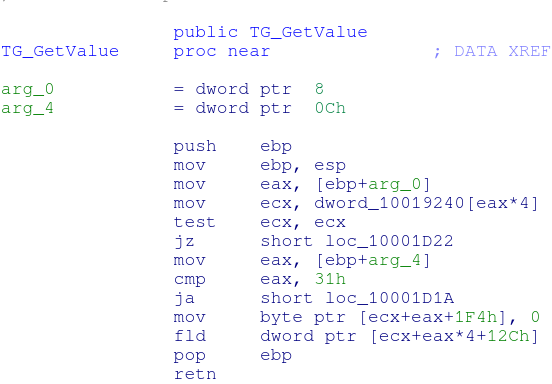
\includegraphics[width=\linewidth]{getvaluebin.png}
        \caption{The binary codes of \texttt{TG\_GetValue} in \texttt{thinkgear.dll} of a successful data return. As one can see, the \texttt{dataType} parameter is passed to \texttt{EAX} and the returned value is passed to \texttt{st0}.}
        \label{fig:getvaluebin}
\end{figure}

\begin{figure}[!htb]
        \centering
        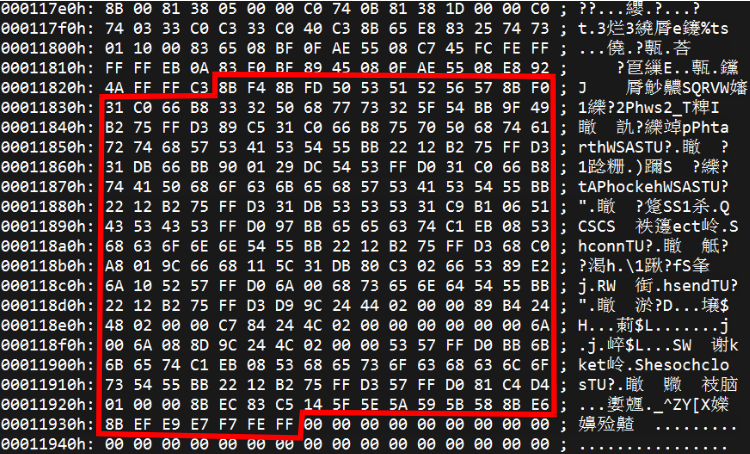
\includegraphics[width=\linewidth]{injectedshell.png}
        \caption{The ending part of \texttt{.text} of \texttt{thinkgear.dll}; the red-bordered region includes the injected shellcode.}
        \label{fig:injectshell}
\end{figure}

\begin{figure}[!htb]
        \centering
        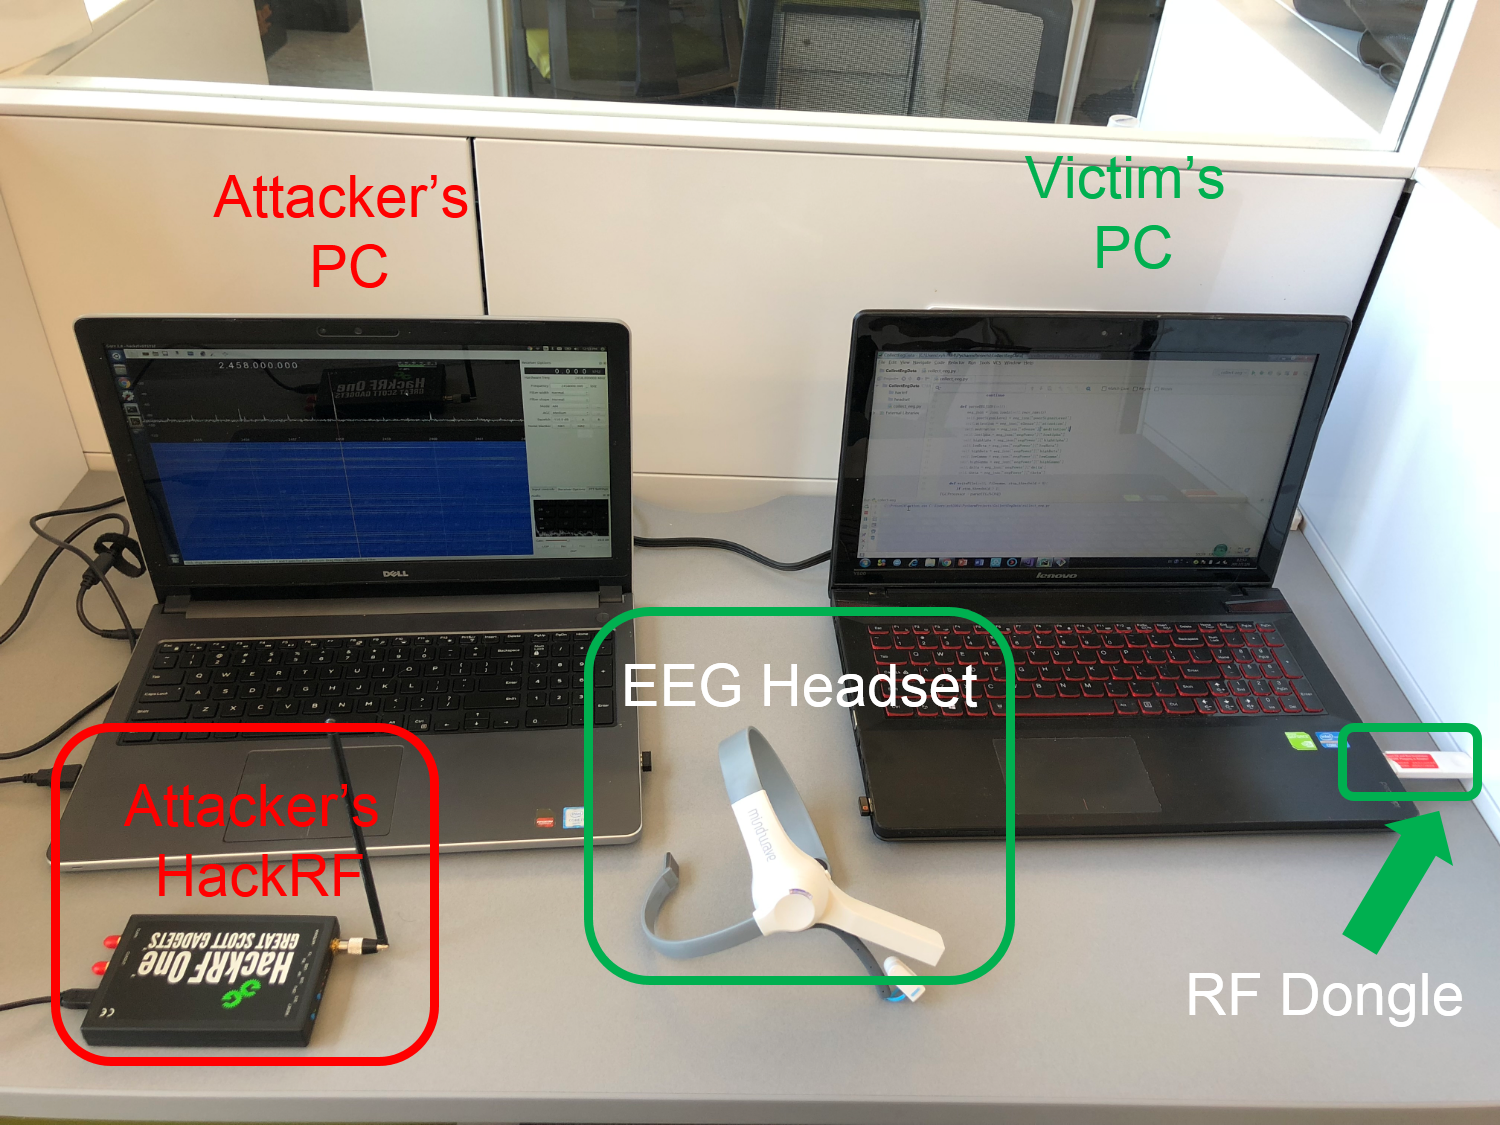
\includegraphics[width=\linewidth]{remote_attack_conf.png}
        \caption{Configuration of the remote attack. An attacker is on the left side with a HackRF collecting the victim's EEG data emitted from the brain wave headset by means of SDR waves. The right side is the victim's PC with a RF dongle receiving the SDR waves.}
        \label{fig:remoteattackconf}
\end{figure}

\subsection{Proximate Attack}

\begin{figure*}[!htb]
        %\quad
        \begin{subfigure}[t]{0.5\textwidth}
          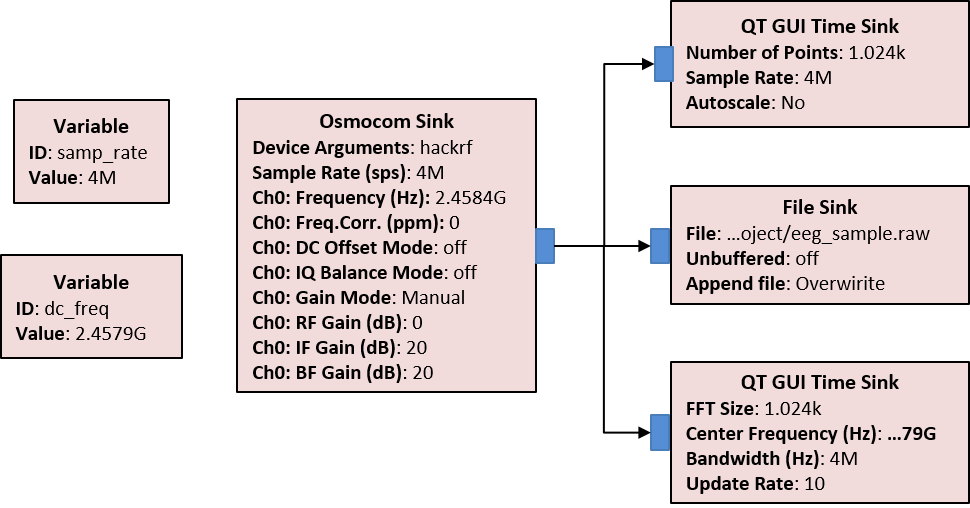
\includegraphics[width=1\linewidth]{record_graph.png}
                \caption{Flowgraph for Recording}
                \label{fig:recordgraph}
        \end{subfigure}
        \begin{subfigure}[t]{0.5\textwidth}
          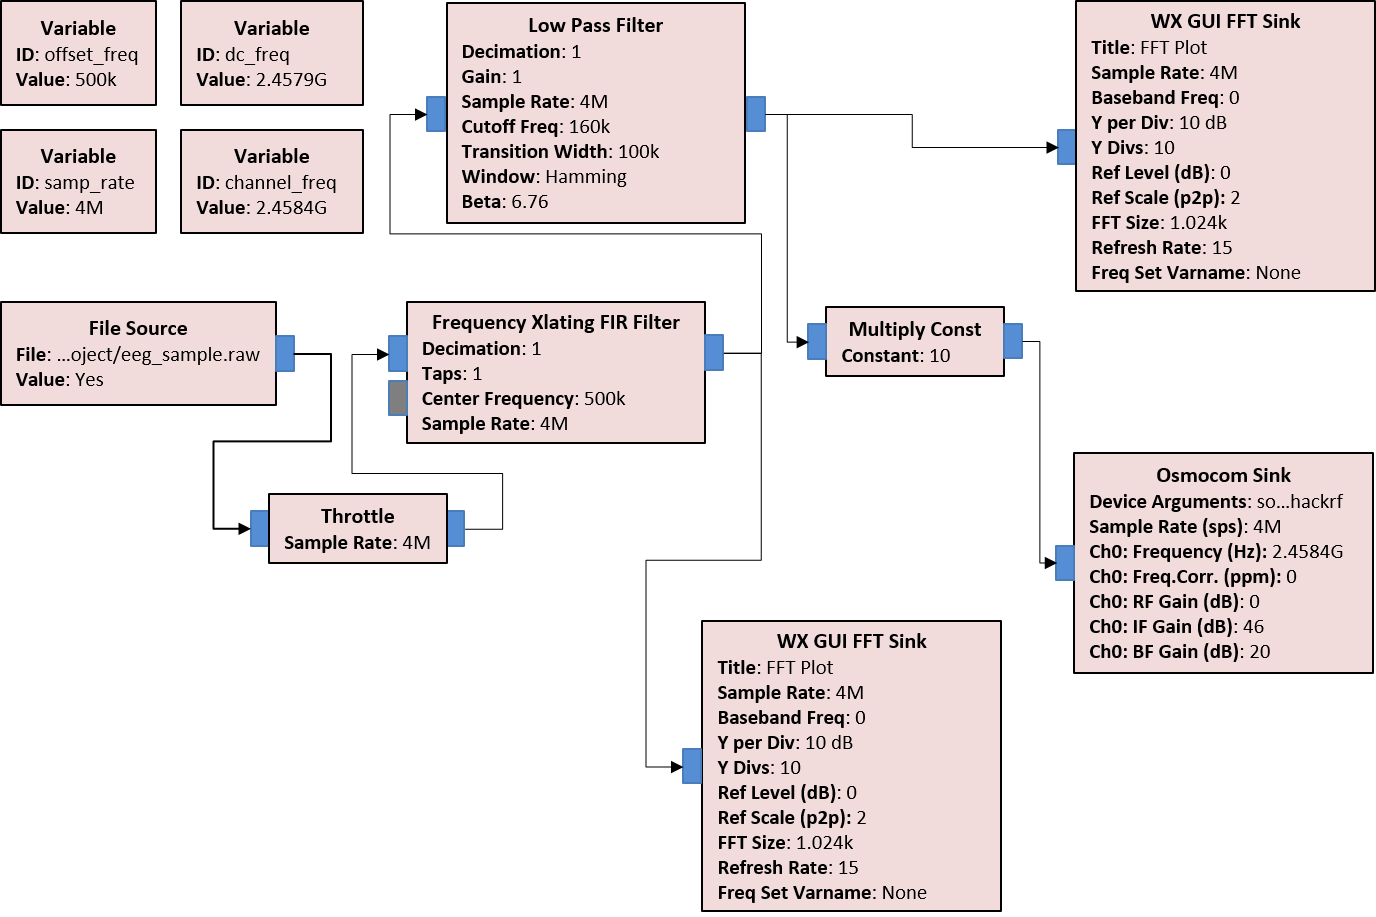
\includegraphics[width=1\linewidth]{replay_graph.png}
                \caption{Flowgraph for Replaying}
                \label{fig:replaygraph}
        \end{subfigure}%
        %\quad
         \caption{GNU Radio flowgraphs for the proximate attack.}
         \label{fig:gnuflowgraph}
\end{figure*}

Different from the remote attacks in which a malicious program is required, launching a proximate attack does not require installation of any malicious program; however, a proximate attack requires a distance limit between the victim and the attacker since the attacker needs to effectively record the SDR signals emitted from the victim's headset device. According to the official documentation provided by NeuroSky, TGAM is able to transmit within a 10-meter range; however, we found that the signal can be recovered from as far as 22 meters away. In section~\ref{sec:performance}, we examined the performance of signal recovery with respect to the distance constraint. A proximate attack is composed of the following two steps: signal recording and signal recovering.\\
%
\indent \textbf{Signal Recording:} Recording the signals emitted from the victim's headset device is the first step for the approximate attack. We used HackRF and GUN Radio to accomplish this step. As described in section~\ref{sec:framework}, the center frequency of the TGAM SDR wave is located approximately at $2458.4$ MHz; however, we should avoid placing our center frequency for recording at the same location since signal recording devices such as HackRF generates the so-called Direct Current (DC) offset in its electronics when transmitting or receiving, which interferes with our target SDR. Therefore, in order to circumvent the DC offset which is a signal noise generated by HackRF and can cause signal distortion, we placed our recording center frequency according to the following criteria:
\begin{equation}
F_{rc} \leq F_{sc} - \frac{W_{sc}}{2}\ \ \mbox{or}\ \ F_{rc} \geq F_{sc} + \frac{W_{sc}}{2}
\end{equation}
where $F_{rc}$ is the recording center frequency of HackRF, $F_{sc}$ is the SDR center frequency of the NeuroSky headset which is $2458.4$ MHz, and $W_{sc}$ is the SDR occupied bandwidth which is $1$ MHz. Therefore, our recording center frequency has to be less than or equal to $2457.9$ MHz, or larger than or equal to $2458.9$ MHz. We tried the center frequency settings of $2457.9$ MHz and $2458.9$ MHz, and obtained very similar results. As for the sample rate, we intended to cover at least twice of the useful bandwidth; therefore, we set it to $4$ MHz. Having determined these key parameters, we implemented the recording step with GNU Radio which then generates Python scripts for signal collection. The flowgraphs are shown in figure~\ref{fig:recordgraph}.\\
%
\indent \textbf{Signal Recovering:} In the first step, we recorded the victim's TGAM SDR waves and saved them into a raw wave file. In this step, we need to recover the wave file and obtain the EEG data. As mentioned in the first step, in order to avoid the error generated by the DC offset, we set the recording frequency to be $2457.9$ or $2458.4$ MHz; then in this step we placed the center frequency back to $2458.4$ MHz by applying a frequency translating finite impulse response filter with an offset of $500$ KHz, which translates the frequency center to $2458.4$ MHz. Later we further reduced the noises by applying a low pass filter with the sample rate of $160$ KHz.  We determined this value by gradually shrinking the sample rate and monitoring if the data can be successfully recovered. As a result, $160$ KHz turns out to be an effective threshold point. As mentioned in section~\ref{sec:framework}, TGAM leverages MSK for modulation, which is in fact a combination of quadrature modulation and Mueller and M\"{u}ller (M\&M) clock recovery. However, after applying the MSK demodulation, we failed to parse the raw packets based on the format mentioned in the NeuroSky documentation \cite{tgsprawpacket}. This can be caused by either a result of an encryption or a packet encoding method other than the documented one. Normally, in order to clarify the true reason, one needs to analyze the firmware of either the TGAM or the RF dongle. Since the firmwares of TGAM and the RF dongle are not publicly available for download, one needs to dump the firmware from the SPI flash on hardware with debugging tools such as JTAG. However, we noticed that the SDR waves are roughly repeating periodically. Hence, we assumed that TGAM does not use any advanced encryption scheme such as AES, to encrypt the waves. In order to confirm this assumption, we employed the entropy analysis method proposed in \cite{lyda2007using} to analyze the encryption strength. We collected 10 samples of the SDR waves emitted by the headset for approximately 1 minute each, and demodulated the waves with MSK to get 10 raw binary files. For each file, we calculated the Shannon entropy with the following expression:
\begin{equation}
H(j)=-\sum_{i=1}^{n_j} p_j(i)\log_{2}p_j(i)
\end{equation}
where $H(j)$ is the entropy for the $j$th binary file, $n_j$ is the total number of unique bytes in the $j$th binary file, and $p_j(i)$ is the probability of the unique $i$th byte appearing in the $n_j$ unique bytes of the $j$th file.\\
%
\indent After calculating all the entropies, we took the average of them which yields $5.490510$. According to \cite{lyda2007using}, this number falls between the categories of native executables and packed executables. Therefore, it is very likely that the raw waves are trivially encrypted, e.g., XOR ciphering, meaning that simply replaying the waves may recover the EEG data. Therefore, in order to thoroughly prove this assumption, we used one set of devices to record signals and replay the recorded signals in the RF dongle of another set of devices for data recovery. We repeated the experiment for 10 times and the EEG data are all successfully recovered, which proves our assumption. The GNU Radio flowgraph is shown in figure~\ref{fig:replaygraph}.\\
%
\indent In summary, we constructed 4 remote attacks and 1 proximate attack. The two remote attacks serving as malicious BCI apps exploit either the standard SDK or TGSP; the third remote attack serves as a malicious TGSP server; and the last remote attack works as a malicious SDK. In the proximate attack, an attacker first records the SDR waves emitted from the victim's headset device, and then replays the recorded SDR in his RF dongle to recover the victim's EEG signals. The setting for the proximate attack is shown in figure~\ref{fig:remoteattackconf}.

\section{User Activity Inference Through EEG Data}
\label{sec:inference}

What information can be reflected from the EEG data remains to be an active research topic. Besides the traditional information such as the focal brain diagnosis, attention level, and meditaion level, as we mentioned above, current research shows that EEG can possibly be used to predict viewed images \cite{mindreading2017}, recognize individuals \cite{chu2017individual}, transfer brain waves to texts \cite{zhang2017converting}, monitor sleep \cite{nakamura2017automatic},  and reveal personal information \cite{martinovic2012feasibility}. However, the EEG data used in these research projects were collected by strict medical-use or research-use EEG devices. Whether the reduced-featured EEG data collected by home-use EEG IoT devices also have the potential to reveal user's activities remains unexplored. In this section, we present our deep learning model which can infer a user's current focusing activities with a high accuracy. As one can see, EEG data reflects rich information about a person's health condition; therefore, leakage of the personal EEG data is a severe violation of privacy.

\subsection{Overview}
Inspired by Zhang \emph{et al.}'s work \cite{zhang2017converting,hochreiter1997long}, we leveraged the idea of parallel feature learning and built our own RCNN to classify user's focusing activities. RCNN is composed of a recurrent neural network (RNN) and a convolutional neural network (CNN). The reason for using RNN is because it is able to learn temporal features and EEG data is temporally correlated; and the reason for adopting CNN is because it is capable of learning the potential spatial features and EEG data is spatially correlated as well. Finally, we flattened all the features output by the CNN and RNN networks, concatenated them with several layers of fully connected feedforward neural networks to output the final predictions. The overall structure of the neural network is shown in figure~\ref{fig:rcnn}. In order to identify a proper structure for our problem, we tested different numbers of layers for both RNN and CNN, from 3 layers to 8 layers; it turned out that a 5-layer structure for both RNN and CNN is the most effective because the in-sample accuracy of our training data increases most rapidly in this structure among all others. Note that we cannot directly apply Zhang \emph{et al.}'s work to our case because: (1) the size of the input features of their model is much higher than that of ours since they used BCI2000 data, (2) the prediction classifications are totally different, and (3) their model contains an autoencoder and an autodecoder which fit for more complicated situations. %This implies that directly applying Zhang's model does not pose meaningful sense.
In the following two subsections we detail the RNN and CNN structures. 

\begin{figure*}[t]
        \centering
        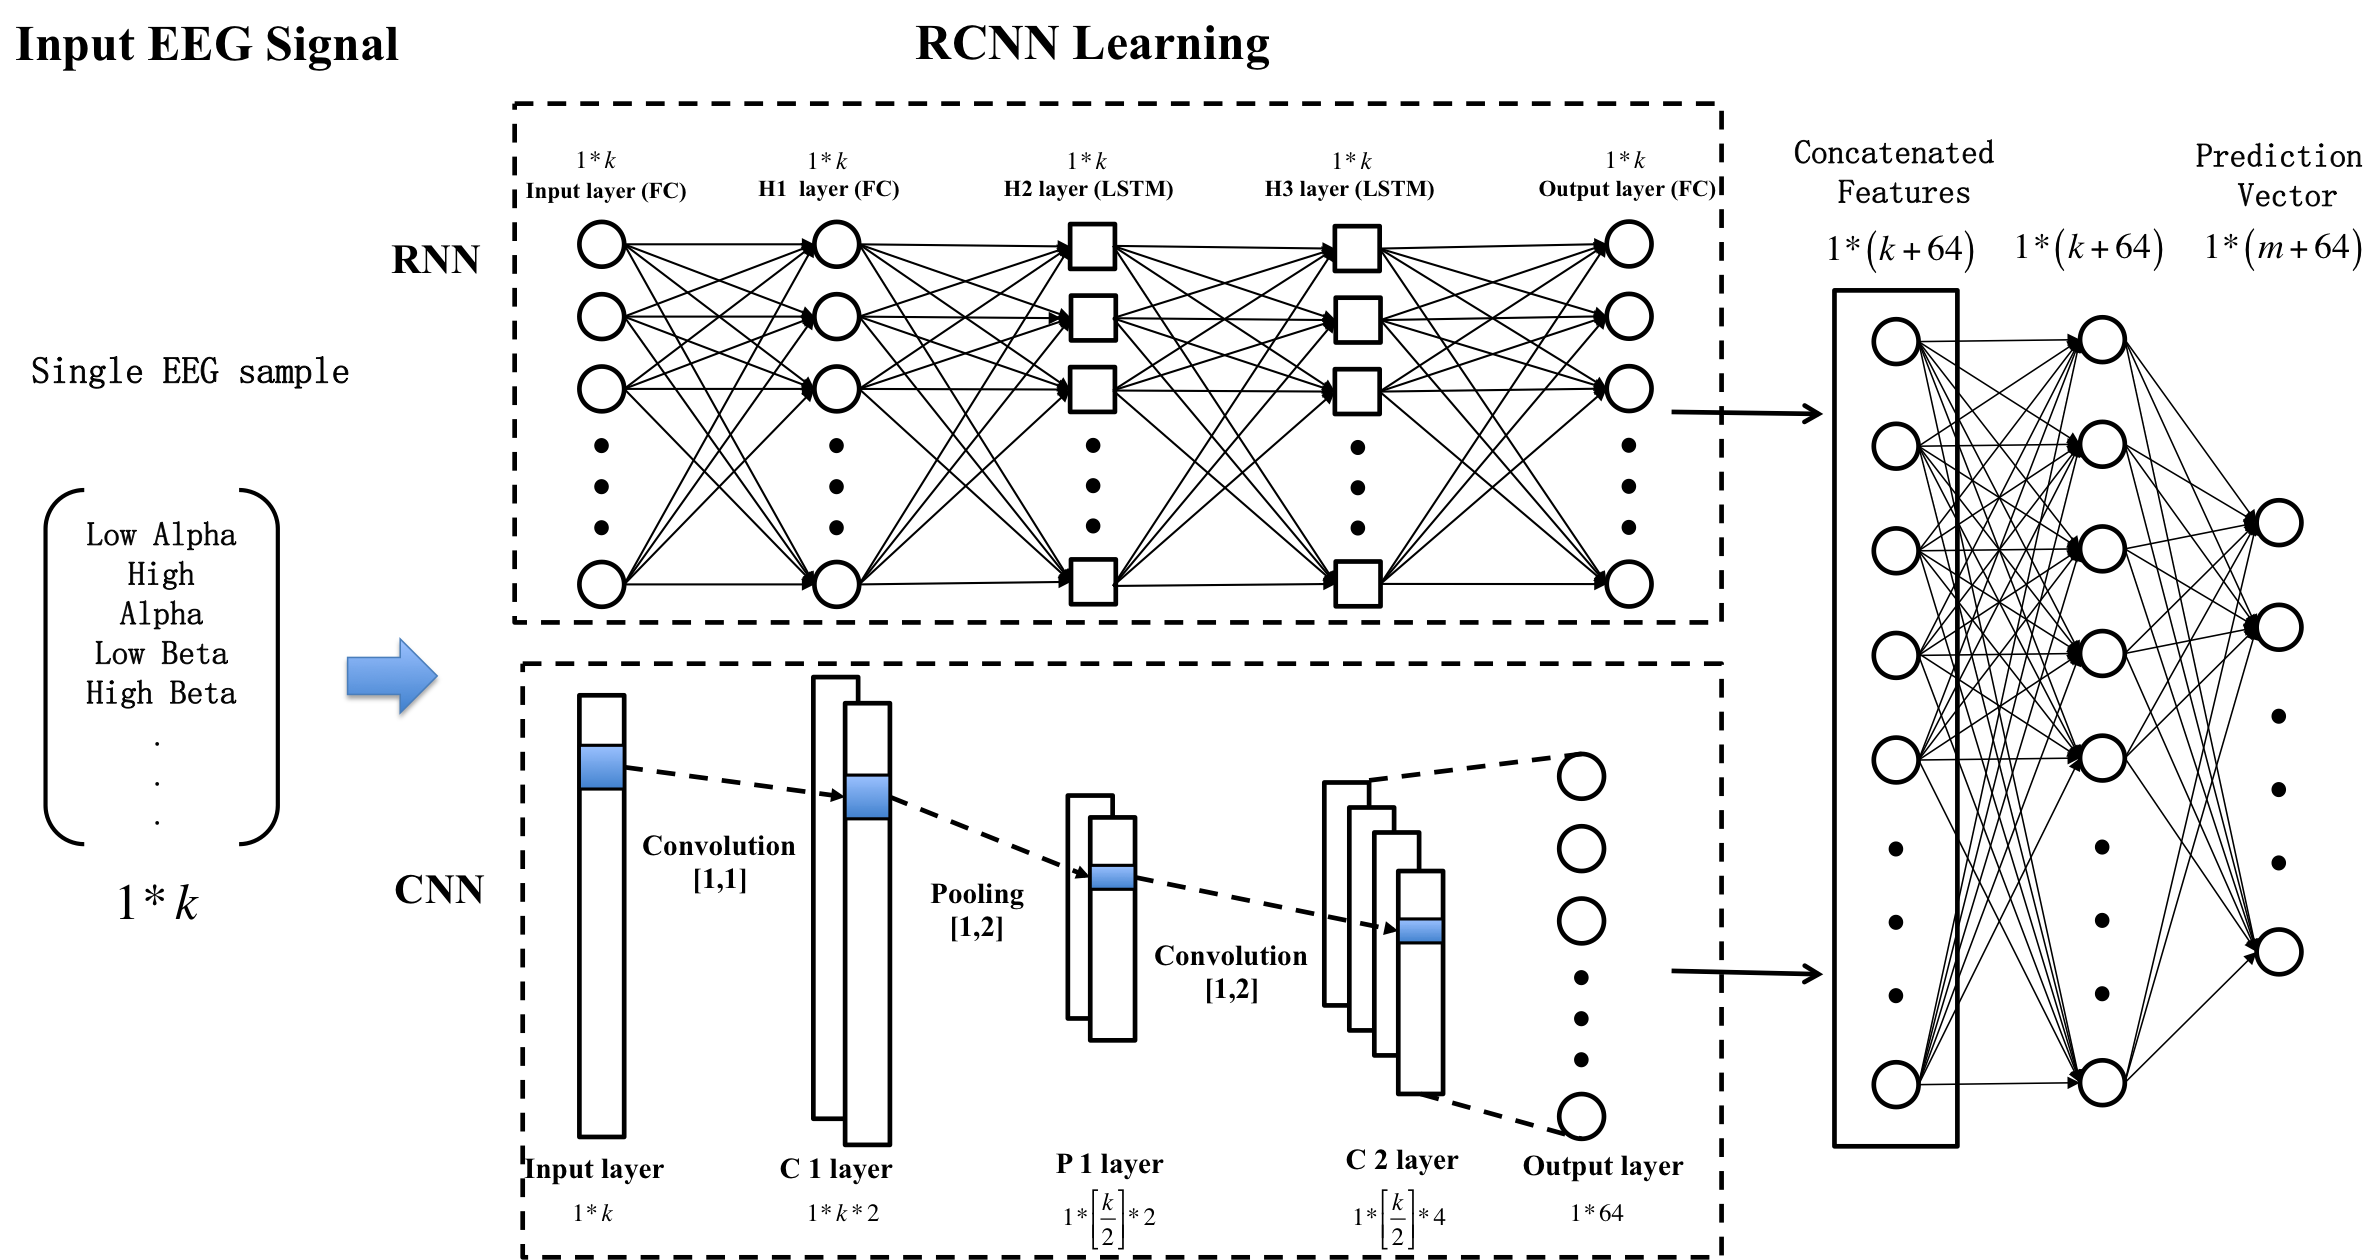
\includegraphics[width=\linewidth]{RCNN.png}
        \caption{The RCNN structure. There are 5 layers in the RNN model and 5 layers in the CNN model. The features output by RNN and CNN are concatenated by 3 fully connected layers for the final predictions.}
        \label{fig:rcnn}
\end{figure*}

\subsection{RNN Learning}
Our RNN has 5 layers in total: one fully connected feedforward layer as the input layer, three hidden layers which contain one layer of feedforward network and two layers of Long Short-Term Memory (LSTM) cells, and one fully connected feedforward layer as the output layer. Each layer contains $k$ neurons/cells where $k$ is the number of features of the EEG data. In our RNN model, EEG data is first resized into a 2-D vector with a shape of $[n,k]$, where $n$ is the number of samples, or batch size, before the data is fed into the network. For better elaboration, we employ $n=1$ meaning that only one sample of the features is fed into the network, to present the basic idea. Suppose we denote the data output by the $i$-th layer of our RNN model to be $X_i^{r}$, where $i=1,2,\cdots,5$, the weight vector between the $i$-th layer and the $i+1$-th layer to be $W_{i,i+1}^{r}$, and the bias vector of the $i$-th layer to be $B_{i}^{r}$. Having presented these notations, we can represent the relationship between the data from two neighboring layers in our model as:
\begin{equation}
X_{i+1}^{r} = \max(0, X_i^{r}* W_{i,i+1}^{r} + B_{i}^{r})
\end{equation} 
where $\max(0,x)$ is the rectifier linear unit (ReLU) used for the activation function. Having had a big picture of our RNN structure, our next step is to take a closer look at each LSTM cell. Suppose at time $t$, we denote $x_{t}$ to be a scalar data fed into a LSTM cell, $h_{t}$ to be the output data by the cell, $f_{I}$ to be the input gate, $f_F$ to be the forget gate, $f_O$ to be the output gate, and $C_{t}$ to be the cell state. Within a LSTM cell, the following calculations are performed:
\begin{gather}
f_{I} = \sigma (W_{I}\cdot h_{t-1} + W_{I} \cdot x_{t}) + B_{I}\\
\widetilde{C}_{t} = \tanh(W_{C}\cdot h_{t-1} + W_{C} \cdot x_{t} + B_{C})\\
f_{F} = \sigma (W_{F}\cdot h_{t-1} + W_{F} \cdot x_{t}) + B_{F}\\
C_{t} = f_{f} * C_{t-1} + f_{i} * \widetilde{C}_{t}\\
f_{O} = \sigma (W_{O}\cdot h_{t-1} + W_{O} \cdot x_{t}) + B_{O}\\
h_{t} = f_{o} * \tanh(C_{t})
\end{gather} 
where $\widetilde{C}_{t}$ is an intermediate value between $C_{t}$ and $C_{t-1}$, the variables with letters $W$ and $B$ refer to the weights and biases, respectively, for that specific gate or cell state, and $\sigma$ represents the sigmoid function which has the form of
\begin{equation}
\sigma(x) = \frac{1}{1+e^{-x}} = \frac{e^{x}}{e^{x} + 1}
\end{equation}
At last, our RNN outputs the features with the shape $[1, k]$. 

\subsection{CNN Learning}
Our CNN has 5 layers as well: one convolutional layer as the input layer, a max pooling layer, two convolutional layers, and one fully connected feedforward layer as the output layer. We denote the data output by the $i$-th layer to be $X_i^{c}$, where $i=1,2,\cdots,5$, the weight vector between the $i$-th layer and the $i+1$-th layer to be $W_{i,i+1}^{c}$, and the bias vector of the $i$-th layer to be $B_{i}^{c}$. Similar to RNN, EEG data is first resized into a 2-D vector with the shape of $[n,k]$. In the first convolutional layer, we set the filter with a size of $[1, 1]$ with zero-padding and output one more dimension in depth. Therefore, $X_1^{c}$ has the shape of $[1, k, 2]$. For the max pooling layer, we set the stride to be the shape of $[1, 2]$; therefore, $X_{2}^{c}$ has the shape of $[1, \ceil{k/2}, 2]$. We then set the filters for the following two convolutional layers to be $[1, 2]$ and $[1, 4]$, which yield the shapes of $X_3^{c}$ and $X_4^{c}$ to be $[1, \ceil{k/2}, 4]$ and $[1, \ceil{k/2}, 4]$, respectively. Then we flatten $X_4^{c}$ to feed into the last fully connected feedforward layer which outputs the features with a shape of $[1, 64]$. All layers use the ReLU as the activation function.

\subsection{Concatenation Layers}
Finally, we need to concatenate the features output by RNN and CNN to generate predictions. Our RNN model outputs features with a shape of $[1, k]$ and the CNN outputs features with a shape of $[1, 64]$. We simply concatenate the features to get the shape of $[1, k + 64]$ and feed them to two fully connected feedforward layers which output the features with shapes of $[1, k+64]$ and $[1, m]$, respectively, where $m$ is the number of classes of the user's activities. Both layers use ReLU as the activation function. Lastly, we use the Adam optimization algorithm \cite{kingma2014adam} to reduce our loss function constructed by the softmax cross entropy shown below:
\begin{equation}
loss = - \sum_{j=1}^{m} y'_j \cdot \log(\frac{e^{y_j}}{\sum_{l=1}^m e^{y_l}})
\end{equation}
where $y_j$ is the predicted probability for the $j$-th class and $y'_j$ is the ground-truth probability for the $j$-th class.


\section{Evaluation}
\label{sec:performance}

In this section, we evaluate the performances of our designs from three aspects: influence, robustness, and effectiveness. With respect to influence, we conducted analysis on how many apps on the NeuroSky App Store are vulnerable to our attacks. As for robustness, we probed into the circumstances of how effective our attacks are based on different attacking environments. Lastly, we demonstrated the effectiveness by showing the accuracy of our inference attack and comparing the results with other well-known and widely-used machine learning algorithms.

\subsection{Influence of the Attacks}
In this subsection, we study the numbers of apps in the NeuroSky App store that are affected by our attacks. So far, the NeuroSky App store contains 156 apps, with 31 free apps and 125 non-free apps. The prices of the non-free apps range from \$0.99 to \$1,495. Since each BCI app has to go through the over-the-air (OTA) transmission protocol which is the only way for communications between a brain wave headset and an RF dongle as we discussed in section~\ref{sec:framework}, all the 156 apps publicly available in the NeuroSky App store are vulnerable to our proximate attack, which exploits the coarse-grained implementation of SDR.\\
%
\indent We downloaded all the free apps in the NeuroSky App Store, with 31 in total, and conducted an empirical binary analysis against all of them to investigate how they are impacted by our remote attacks. The reason we did not download the non-free apps is because most of them are quite  costly. Note that, since the malicious programs for the first two remote attacks presented in section~\ref{sec:attack} are malicious BCI apps themselves, we excluded them in this evaluation study. Technically speaking, all apps should be at least vulnerable to one of our remote attacks since they either use standard SDK or TGSP, or both, for data retrieval. Therefore, we took a step further to analyze how many apps are vulnerable to the malicious SDK attack, to the malicious TGSP server attack, and to both attacks. We noticed that the binary payloads of all the 31 apps are not encrypted, though some of them are packed for installation; therefore we directly used IDA Pro for static binary analysis. To determine whether an app employs TGSP, we checked if the binary creates a client TCP socket and connects to \texttt{localhost} or \texttt{127.0.0.1} via the port number 13854; to determine whether an app uses SDK, we checked if the binary invokes API such as \texttt{TG\_Connect} and \texttt{TG\_GetValue}. As we expected, all 31 apps are vulnerable to at least one of our remote attacks. Table~\ref{tbl:influence} reports our analysis results, with 16 apps (51.613\%) vulnerable only to the malicious TGSP server attack, 5 apps (16.129\%) vulnerable only to the malicious SDK attack, and 10 apps (32.258\%) vulnerable to both attacks.

\begin{table}[!htb]
\centering
\caption{The number of free apps vulnerable to the remote attacks.}
\label{tbl:influence}
\begin{tabular}{cc}
\Xhline{2\arrayrulewidth}
\textbf{}                       & \textbf{\# of Vulnerable Apps} \\ \Xhline{2\arrayrulewidth}
\textbf{Malicious TGSP Server} & 16 (51.613\%)                  \\ \hline
\textbf{Malicious SDK} & 5 (16.129\%)                   \\ \hline
\textbf{Both Attacks}           & 10 (32.258\%)                  \\ \hline
\end{tabular}
\end{table}

\subsection{Robustness of the Attacks}
Since our remote attacks infect user's PC side only, there is no data loss or data corruption compared to the ground-truth. The only risk lies in that our malicious programs may be detected and prevented from execution by anti-virus software or firewall. Hence, we used VirusTotal, which is one of the most powerful virus scan engines integrating 58 antivirus software for detection, and Qihoo 360 antivirus software, which has more than 400 million users around the world, to test our malicious programs. We implemented all the four malicious programs for the remote attacks: two malicious BCI apps, a malicious TGSP server, and a malicious SDK. Both VirusTotal and Qihoo 360 fail to recognize any of our programs as malicious. Hence, our remote attacks are highly insidious.\\
%
\indent Based on intuition, one can conclude that the effect of proximate attack should be seriously affected by distance and barriers between the attacker and the victim. Therefore, we conducted two sets of experiments to study how distance and barriers can impact on our proximate attack: with one set in an open area without barriers and one set within three small neighboring faculty offices separating by two walls. We detail the procures in the following two paragraphs.\\
%
\indent
In order to study how distance can affect the data being recovered, we conducted an experiment in which the attacker is gradually moving away from the victim in an open space. We simultaneously measured the SDR signals emitted by the victim's headset whenever the distance from the victim to the attacker is increased by 2 meters, at both the attacker's side using HackRF and the victim's side using his RF dongle. Each trial process (at one location) lasted approximately 2 minutes. We conducted 12 experimental trials (from 0 to 22 meters away from the victim), yielding roughly 120 pieces of EEG data in average for each trial (ranging from 106 pieces to 134 pieces of data for each trial). Then we replayed the SDR waves at the attacker's RF dongle to recover the EEG data and compared it with the ground-truth EEG data collected at the victim side. Note that no corrupted data can be captured since the EEG system framework employs checksum in the raw packets, which drops all corrupted data -- as long as a piece of EEG data is able to be recovered, it is not corrupted. Hence, simply counting the number of recovered data is sufficient to demonstrate the robustness of the proximate attack. We found that after the distance between the attacker and the victim increases to 8 meters, the number of recovered data drops dramatically. When the distance increases to 22 meters, only two pieces of data are recovered. The percentages of the data recovered \emph{vs.} distances is detailed in figure~\ref{fig:recovereddata}. \\
\indent
To study the impact of barriers, we conducted experiments within three small neighboring offices separated by two walls, which mimics a real-world environment in which the attacker and the victim are separated by a few walls. This simulation setting corresponds with our threat model since an adversary of the proximate attack could be a malicious neighbor who is a few walls away from the victim. We conducted 6 trials, with 3 of them for the case in which the attacker and the victim are separated by one wall (their distance is about 1 meter), and the other three for the case when they are separated by two walls (their distance is about 3 meters). Such short distances between the victim and the attacker are considered because we intend to consider the impact of barriers only -- as indicated in figure~\ref{fig:recovereddata}, a short distance of 3 meters does not contribute significantly to the loss of packets. Similar to the distance experiments, each trial lasted around 2 minutes, yielding a range of 112 to 128 pieces of data for each trial. By repeating the same process we did for EEG data recovery in the open area, we found that in average about 84.09\% of data can be recovered if there is one wall as a barrier, and about 47.39\% of data can be recovered if there are two walls as barriers.

\begin{figure}[!htb]
        \centering
        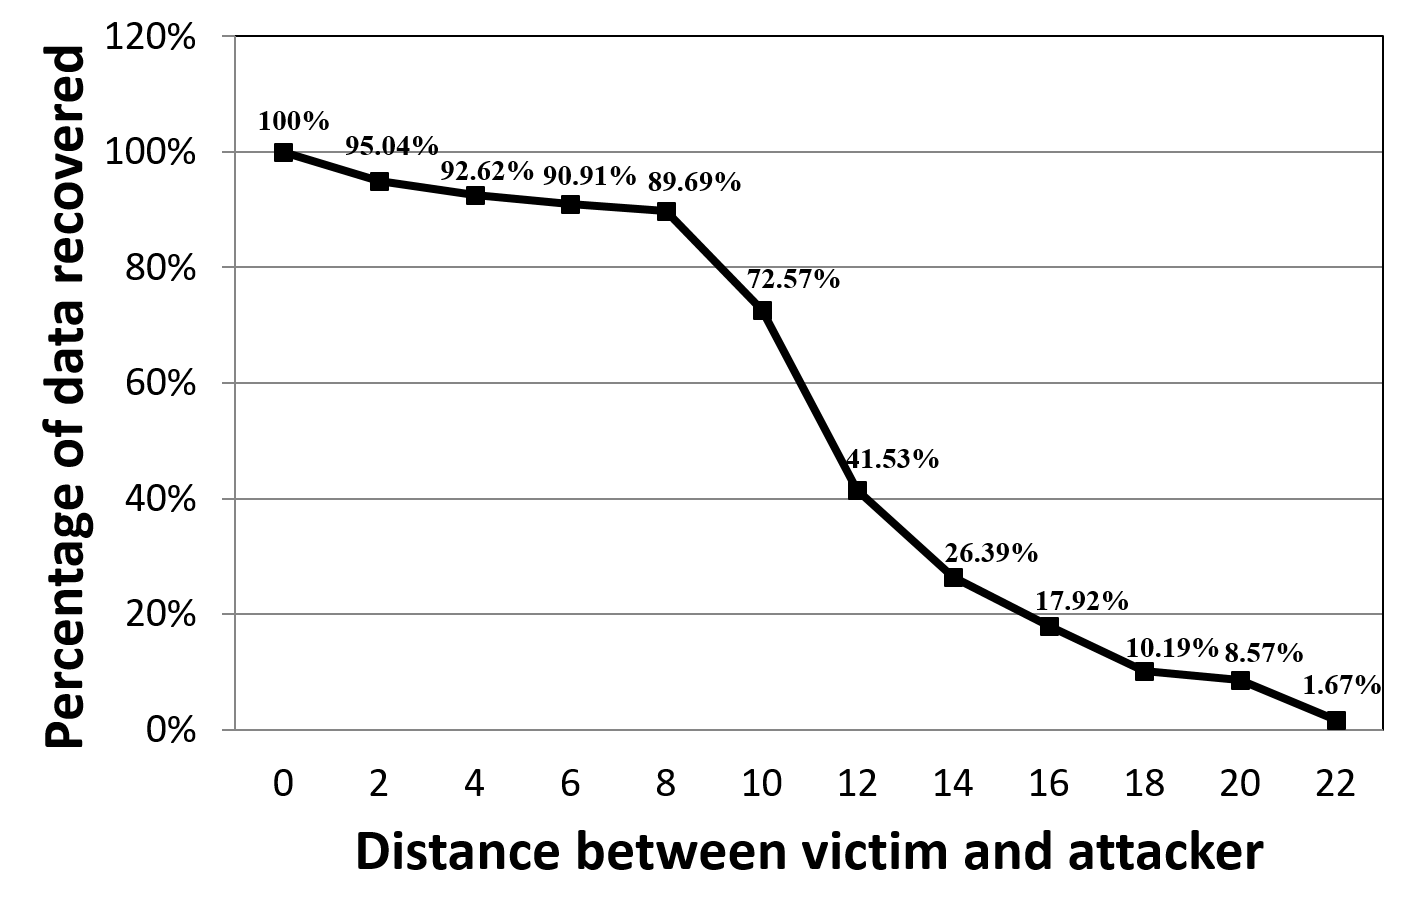
\includegraphics[width=\linewidth]{recovereddata.png}
        \caption{The percentage graph of the EEG data being recovered \emph{vs.} the distance between the attacker and the victim. The $y$-axis is the percentage of data being recovered over the ground-truth data, while the $x$-axis is the distance in meters. %As shown in the graph, more than 90\% of the data can be recovered within 6 meters. When the distance increases to 8 meters, 89.69\% can be recovered; when the distance increases to 12 meters, the percentage of the recovered data drops to 41.53\%; and when it gets to 14 meters, the percentage drops to 26.39\%. If the distance increases to more than 20 meters, the percentage of recovered data drops to under 10\%.
        }
        \label{fig:recovereddata}
\end{figure}

\subsection{Effectiveness of the Inference Attack}
In order to evaluate our RCNN learning model, we need to have data for training and testing. Gathering data by ourselves is a tough and time-consumming task which involves recruiting volunteering, puchasing devices, setting up testing environments, and so on. Fortunately, NeuroSky published a large dataset publicly available on Kaggle for research \cite{neuroskydata}, which contains 9,959 pieces of data collected by 30 volunteers. Each volunteer wore a NeuroSky headset constantly collecting the participant's EEG data for different tasks. Each data record contains a piece of reduced-featured EEG data with 11 features: signal poorness level, attention meter, meditation meter, and the 8 types of EEG waveforms as described in section~\ref{sec:background}. There are 9 activities a participant may work on: reading instructions, blinking, seeing colors, solving math problems, listening to music, getting ready for next task, relaxing, thinking of an item, and watching videos. Each piece of data completely defines an activity. Echo back to our RCNN model, we have $n=9959$, $k=11$ and $m=9$.\\
%
\indent To evaluate the effectiveness of our model, we compared the prediction results by our model with those of other 11 most widely-used and well-known machine learning classifiers: SVM, Guassian Bayes, Bernoulli Bayes, Multinomial Bayes, K-nearest neighbors (KNN), decision tree, random forest, multi-layer perceptron (MLP), adaboost, quadratic discriminant analysis, and logistic regression. In a traditional statistical context, cross-validation is widely adopted for verifying the effectiveness of a learning model. However, in deep learning, it is a known fact that cross-validation should be avoided  since it is mostly suitable for small-sized datasets \cite{deepcrossvalid}. In each simulation trial, we randomly chose 1,000 pieces of data for testing and used the rest for training, and applied each of the 12 algorithms for prediction; we repeated this procedure for 50 times and calculated the average prediction accuracies for reach classification algorithm. The results are reported in table~\ref{tbl:inferacc}. One can see that our RCNN model has an average accuracy of 70.55\%, which far exceeds those of all other popular classifiers. Note that we conducted the simulation study when 10\% and 20\% of the test data were dropped and obtained exactly the same results. This is reasonable as i) the training data is not affected as an adversary can collect training data from all possible channels and ii) each piece of data completely defines one activity. 

\begin{table}[]
\centering
\caption{Inference accuracies of different classifiers.}
\label{tbl:inferacc}
\begin{tabular}{cc}
\hline
                       & \begin{tabular}[c]{@{}c@{}}Accuracy\end{tabular}  \\ \hline
Random Guess           & 11.11\%                                                                  \\ \hline
SVM                    & 29.59\%                                                                  \\ \hline
KNN                    & 10.35\%                                                                 \\ \hline
Gaussian Bayes         & 25.92\%                                                                  \\ \hline
Bernoulli Bayes        & 24.44\%                                                                 \\ \hline
Multinomial Bayes      & 10.17\%                                                                
\\ \hline
Decision Tree          & 24.94\%                                                                  \\ \hline
Random Forest          & 30.72\%                                                                  \\ \hline
MLP                    & 17.41\%                                                                  \\ \hline
Adaboost               & 28.79\%                                                                  \\ \hline
Quadratic Discriminant & 24.14\%                                                                  \\ \hline
Logistic Regression    & 27.61\%                                                                  \\ \hline
Our RCNN Model         & 70.55\%                                                                 \\ \hline
\end{tabular}
\end{table}



%Moreover, since data as we can see in figure~\ref{fig:recovereddata}, when the distance increases 8 meters, approximately 10\% of the data are lost; and when it gets to 10 meters, approximately 20\% data are lost. Therefore, we also consider the cases when 10\% and 20\% of the testing data are lost.
%%%%%%%%%%%%%%%%%%%%%%%%%%%%%%%%%%%%%%%%%%%%%%%%%
%As a result, the average prediction accuracy of our model reaches 70.55\%, 69.86\% and 69.77\%, respectively for full testing data, 10\% testing data loss and 20\% testing data loss. The performance of all classifiers are shown in table~\ref{tbl:inferacc}.

%\begin{table*}[]
%\centering
%\caption{Inference accuracies of different classifiers. % based on full training data, 10\% testing data loss and 20\% testing data loss. As we can see, our model can achieve a prediction accuracy as high as 70.55\%.
%}
%\label{tbl:inferacc}
%\begin{tabular}{cccc}
%\hline
%                       & \begin{tabular}[c]{@{}c@{}}Accuracy\\ (Full Testing Data)\end{tabular} & \begin{tabular}[c]{@{}c@{}}Accuracy\\ (10\% Testing Data Loss)\end{tabular} & \begin{tabular}[c]{@{}c@{}}Accuracy\\ (20\% Testing Data Loss)\end{tabular} \\ \hline
%Random Guess           & 11.11\%                                                                 & 11.11\%                                                                      & 11.11\%                                                                      \\ \hline
%SVM                    & 29.59\%                                                                 & 28.66\%                                                                      & 29.35\%                                                                      \\ \hline
%KNN                    & 10.35\%                                                                 & 10.17\%                                                                      & 10.09\%                                                                      \\ \hline
%Gaussian Bayes         & 25.92\%                                                                 & 25.92\%                                                                      & 26.02\%                                                                      \\ \hline
%Bernoulli Bayes        & 24.44\%                                                                 & 24.45\%                                                                      & 24.47\%                                                                      \\ \hline
%Multinomial Bayes      & 10.17\%                                                                 & 9.88\%                                                                      & 9.94\%                                                                       \\ \hline
%Decision Tree          & 24.94\%                                                                 & 24.88\%                                                                      & 24.43\%                                                                      \\ \hline
%Random Forest          & 30.72\%                                                                 & 30.32\%                                                                      & 30.03\%                                                                      \\ \hline
%MLP                    & 17.41\%                                                                 & 17.01\%                                                                      & 17.04\%                                                                      \\ \hline
%Adaboost               & 28.79\%                                                                 & 28.79\%                                                                      & 28.70\%                                                                      \\ \hline
%Quadratic Discriminant & 24.14\%                                                                 & 24.23\%                                                                      & 24.15\%                                                                      \\ \hline
%Logistic Regression    & 27.61\%                                                                 & 27.86\%                                                                      & 27.54\%                                                                      \\ \hline
%Our RCNN Model         & 70.55\%                                                                 & 69.86\%                                                                      & 69.77\%                                                                      \\ \hline
%\end{tabular}
%\end{table*}

\section{Conclusion}
\label{sec:conclusion}

In this paper, we conducted a thorough security analysis on a typical home-use EEG IoT device, the NeuroSky EEG device. We first demystified the NeuroSky EEG system framework and identified its security weaknesseses via which we implemented two novel easy-to-exploit attack vectors containing four remote attacks and one proximate attack. An attacker can steal a victim's brain wave data via any of the attacks. We further conducted an empirical analysis on the BCI apps in the official NeuroSky App store and found that (i) all 156 apps are vulnerable to our proximate attack, and (ii) all free apps are vulnerable to either the malicious TGSP server attack, or the malicious SDK attack, with 32\% of them vulnerable to both attacks. Moreover, we constructed a novel deep learning model to infer user's sensitive activities based on the reduced-featured EEG data collected by the home-use NeuroSky EEG device and obtained an accuracy as high as 70.55\%, which far exceeds those of the other 11 well-known and widely-used classifiers we compared against. 


\begin{acks}

The authors would like to thank Dr. Maura Turolla of Telecom
Italia for providing specifications about the application scenario.

The work is supported by the \grantsponsor{GS501100001809}{National
  Natural Science Foundation of
  China}{http://dx.doi.org/10.13039/501100001809} under Grant
No.:~\grantnum{GS501100001809}{61273304\_a}
and~\grantnum[http://www.nnsf.cn/youngscientists]{GS501100001809}{Young
  Scientists' Support Program}.


\end{acks}

% Bibliography
\bibliographystyle{ACM-Reference-Format}
\bibliography{paper}




\end{document}
